\documentclass[twoside]{book}

% Packages required by doxygen
\usepackage{fixltx2e}
\usepackage{calc}
\usepackage{doxygen}
\usepackage[export]{adjustbox} % also loads graphicx
\usepackage{graphicx}
\usepackage[utf8]{inputenc}
\usepackage{makeidx}
\usepackage{multicol}
\usepackage{multirow}
\PassOptionsToPackage{warn}{textcomp}
\usepackage{textcomp}
\usepackage[nointegrals]{wasysym}
\usepackage[table]{xcolor}

% Font selection
\usepackage[T1]{fontenc}
\usepackage[scaled=.90]{helvet}
\usepackage{courier}
\usepackage{amssymb}
\usepackage{sectsty}
\renewcommand{\familydefault}{\sfdefault}
\allsectionsfont{%
  \fontseries{bc}\selectfont%
  \color{darkgray}%
}
\renewcommand{\DoxyLabelFont}{%
  \fontseries{bc}\selectfont%
  \color{darkgray}%
}
\newcommand{\+}{\discretionary{\mbox{\scriptsize$\hookleftarrow$}}{}{}}

% Page & text layout
\usepackage{geometry}
\geometry{%
  a4paper,%
  top=2.5cm,%
  bottom=2.5cm,%
  left=2.5cm,%
  right=2.5cm%
}
\tolerance=750
\hfuzz=15pt
\hbadness=750
\setlength{\emergencystretch}{15pt}
\setlength{\parindent}{0cm}
\setlength{\parskip}{3ex plus 2ex minus 2ex}
\makeatletter
\renewcommand{\paragraph}{%
  \@startsection{paragraph}{4}{0ex}{-1.0ex}{1.0ex}{%
    \normalfont\normalsize\bfseries\SS@parafont%
  }%
}
\renewcommand{\subparagraph}{%
  \@startsection{subparagraph}{5}{0ex}{-1.0ex}{1.0ex}{%
    \normalfont\normalsize\bfseries\SS@subparafont%
  }%
}
\makeatother

% Headers & footers
\usepackage{fancyhdr}
\pagestyle{fancyplain}
\fancyhead[LE]{\fancyplain{}{\bfseries\thepage}}
\fancyhead[CE]{\fancyplain{}{}}
\fancyhead[RE]{\fancyplain{}{\bfseries\leftmark}}
\fancyhead[LO]{\fancyplain{}{\bfseries\rightmark}}
\fancyhead[CO]{\fancyplain{}{}}
\fancyhead[RO]{\fancyplain{}{\bfseries\thepage}}
\fancyfoot[LE]{\fancyplain{}{}}
\fancyfoot[CE]{\fancyplain{}{}}
\fancyfoot[RE]{\fancyplain{}{\bfseries\scriptsize Generated by Doxygen }}
\fancyfoot[LO]{\fancyplain{}{\bfseries\scriptsize Generated by Doxygen }}
\fancyfoot[CO]{\fancyplain{}{}}
\fancyfoot[RO]{\fancyplain{}{}}
\renewcommand{\footrulewidth}{0.4pt}
\renewcommand{\chaptermark}[1]{%
  \markboth{#1}{}%
}
\renewcommand{\sectionmark}[1]{%
  \markright{\thesection\ #1}%
}

% Indices & bibliography
\usepackage{natbib}
\usepackage[titles]{tocloft}
\setcounter{tocdepth}{3}
\setcounter{secnumdepth}{5}
\makeindex

% Hyperlinks (required, but should be loaded last)
\usepackage{ifpdf}
\ifpdf
  \usepackage[pdftex,pagebackref=true]{hyperref}
\else
  \usepackage[ps2pdf,pagebackref=true]{hyperref}
\fi
\hypersetup{%
  colorlinks=true,%
  linkcolor=blue,%
  citecolor=blue,%
  unicode%
}

% Custom commands
\newcommand{\clearemptydoublepage}{%
  \newpage{\pagestyle{empty}\cleardoublepage}%
}

\usepackage{caption}
\captionsetup{labelsep=space,justification=centering,font={bf},singlelinecheck=off,skip=4pt,position=top}

%===== C O N T E N T S =====

\begin{document}

% Titlepage & ToC
\hypersetup{pageanchor=false,
             bookmarksnumbered=true,
             pdfencoding=unicode
            }
\pagenumbering{alph}
\begin{titlepage}
\vspace*{7cm}
\begin{center}%
{\Large P2\+P-\/contract }\\
\vspace*{1cm}
{\large Generated by Doxygen 1.8.14}\\
\end{center}
\end{titlepage}
\clearemptydoublepage
\pagenumbering{roman}
\tableofcontents
\clearemptydoublepage
\pagenumbering{arabic}
\hypersetup{pageanchor=true}

%--- Begin generated contents ---
\chapter{Main Page}
\label{index}\hypertarget{index}{}\label{index_md_README}%
\Hypertarget{index_md_README}%
\doxysubsection*{Стек\+: C/\+C++, eosio.\+cdt 1.\+7.\+0}

\doxysection*{Введение}

Контракт обеспечивает обмен токенами между двумя пользователями системы с участием гаранта. Создавая ордер типа sell, токены продавца блокируются в контракте и передаются покупателю после подтверждения завершения сделки.

Каждый ордер, не обладающий родителем, готов принимать предложения о сделках в дочерних ордерах противоположного типа. Так, если родительский ордер типа buy, то он готов принимать предложения от ордеров с типом sell, и наоборот. Обмен производится по курсу относительно системной опорной валюты (USD).

В процессе обмена всегда задействованы три типа валют\+:
\begin{DoxyItemize}
\item root\+\_\+asset -\/ токен обмена, который предоставляет продавец для блокировки в контракте и получает покупатель после завершения сделки.
\item quote\+\_\+asset -\/ опорный токен, который используется для расчёта количества валюты выхода.
\item out\+\_\+asset -\/ токен выхода, который получает продавец и отправляет покупатель на реквизиты продавца.
\end{DoxyItemize}

\doxysection*{Применение}

Контракт может использоваться\+:
\begin{DoxyItemize}
\item как \mbox{\hyperlink{classp2p}{p2p}} биржа обмена любым стандартным заменяемым цифровым активом;
\item как точка реализации токена компанией (IDO), которая не исключает возможность перепродаж токенов пользователями;
\item как касса взаимопомощи, где только те пользователи могут получить валюту выхода на свои реквизиты, которые обладают токенами обмена; Во всех вариантах каждый хост цифровой экономики на аккаунте \+\_\+core может создать дополнительный стимул на продаже собственных токенов, активировав партнёрскую программу. Для этого, он должен пополнить бонусный баланс контракта и установить бонусный курс, который будет использоваться при расчёте вознаграждений по структуре покупателя по формуле\+: 
\begin{DoxyCode}{0}
\DoxyCodeLine{КОЛИЧЕСТВО\_ТОКЕНОВ\_ПАРТНЁРАМ\_ПОКУПАТЕЛЯ = КОЛИЧЕСТВО\_ТОКЕНОВ\_В\_УСПЕШНОЙ\_СДЕЛКЕ\_У\_ПРОДАВЦА * БОНУСНЫЙ\_КУРС\_ПРОДАВЦА}

\end{DoxyCode}

\end{DoxyItemize}

\doxysection*{Действующие аккаунты}

me -\/ собственное имя контракта; curator -\/ дефолтный оракул, используемый во всех сделках; rater -\/ имя аккаунта поставщика курсов обмена; core -\/ имя аккаунта, распределяющего партнерское вознаграждение;

\doxysection*{Основные управляющие параметры}

ENABLE\+\_\+\+GROWHT = TRUE -\/ допускает изменение курса системного токена в процентном соотношении от стартового курса (линейный рост) START\+\_\+\+RATE -\/ стартовый курс системного токена, используемый при расчёте линейного роста; PERCENTS\+\_\+\+PER\+\_\+\+MONTH -\/ устанавливает скорость роста системного токена; ENABLE\+\_\+\+VESTING -\/ включает режим продаж через вестинг равными долями от момента создания объекта; VESTING\+\_\+\+SECONDS -\/ продолжительность вестинга; CORE\+\_\+\+SALE\+\_\+\+ACCOUNT -\/ аккаунт компании, осуществляющий IDO, продажа от которого проходит с применением вестинга. Все остальные аккаунты совершают сделки без вестинга; GIFT\+\_\+\+ACCOUNT\+\_\+\+FROM\+\_\+\+AMOUNT -\/ если покупка совершается у компании на сумму, превышающую в этом поле, то компания совершает выкуп прав владельца аккаунта у регистратора и передаёт их пользователю (переводит аккаунт из статуса гость в статус партнёр).

\doxysection*{Компиляция}

Заменить ABSOLUTE\+\_\+\+PATH\+\_\+\+TO\+\_\+\+CONTRACT на абсолютный путь к директории контракта \mbox{\hyperlink{classp2p}{p2p}}. 
\begin{DoxyCode}{0}
\DoxyCodeLine{docker run -\/-\/rm -\/-\/name eosio.cdt\_v1.7.0 -\/-\/volume /ABSOLUTE\_PATH\_TO\_CONTRACT:/project -\/w /project eostudio/eosio.cdt:v1.7.0 /bin/bash -\/c "{}eosio-\/cpp -\/abigen -\/I include -\/R include -\/contract p2p -\/o p2p.wasm p2p.cpp"{} \&}

\end{DoxyCode}


\doxysection*{Роли}


\begin{DoxyItemize}
\item Продавец -\/ создаёт ордер типа sell
\item Покупатель -\/ создаёт ордер типа buy
\item Оракул -\/ разрешает споры между партнёрами
\item Поставщик курса -\/ поставляет курс валют выхода
\item Системный поставщик курса -\/ поставляет курс системной валюты
\end{DoxyItemize}

\doxysection*{Сценарии}

\doxysubsubsection*{Пополнение собственного баланса}

Для того, чтобы иметь возможность создать ордер на продажу, необходимо обладать балансом на контракте. Для этого, необходимо совершить перевод на имя аккаунта контракта без дополнительных параметров в поле memo\+: 
\begin{DoxyCode}{0}
\DoxyCodeLine{cleos transfer username p2p "{}100.0000 FLOWER"{}}

\end{DoxyCode}
 Проверить собственный баланс с помощью команды\+: 
\begin{DoxyCode}{0}
\DoxyCodeLine{cleos get table p2p username balance}

\end{DoxyCode}
 Ответ содержит имя контракта и количество токенов, доступных к сделке продажи\+: 
\begin{DoxyCode}{0}
\DoxyCodeLine{"{}rows"{}: [\{}
\DoxyCodeLine{      "{}id"{}: 0,}
\DoxyCodeLine{      "{}contract"{}: "{}eosio.token"{},}
\DoxyCodeLine{      "{}quantity"{}: "{}100.0000 FLOWER"{}}
\DoxyCodeLine{    \}}
\DoxyCodeLine{  ],}

\end{DoxyCode}


\doxysubsubsection*{Пополнение бонусного баланса}

Для пополнения бонусного баланса необходимо совершить перевод на собственное имя аккаунта контракта с указанием в поле memo имени аккаунта, который активирует бонусную систему. Бонусная система доступна только хостам цифровых экономик в контракте core. Аккаунты, не обладающие статусом хоста в контракте core не смогут распределить бонусные токены на структуру покупателя.


\begin{DoxyCode}{0}
\DoxyCodeLine{cleos transfer username p2p "{}100.0000 FLOWER"{} "{}username"{}}

\end{DoxyCode}


Проверить бонусный баланс с помощью команды\+: 
\begin{DoxyCode}{0}
\DoxyCodeLine{cleos get table p2p p2p bbonuses}

\end{DoxyCode}
 Ответ содержит имена аккаунтов хостов и их бонусные балансы\+: 
\begin{DoxyCode}{0}
\DoxyCodeLine{"{}rows"{}: [\{}
\DoxyCodeLine{      "{}host"{}: "{}alexant"{},}
\DoxyCodeLine{      "{}contract"{}: "{}eosio.token"{},}
\DoxyCodeLine{      "{}total"{}: "{}200.0000 FLOWER"{},}
\DoxyCodeLine{      "{}available"{}: "{}200.0000 FLOWER"{},}
\DoxyCodeLine{      "{}distributed"{}: "{}0.0000 FLOWER"{},}
\DoxyCodeLine{      "{}distribution\_rate"{}: "{}0.00000000000000000"{}}
\DoxyCodeLine{    \},\{}
\DoxyCodeLine{      "{}host"{}: "{}core"{},}
\DoxyCodeLine{      "{}contract"{}: "{}eosio.token"{},}
\DoxyCodeLine{      "{}total"{}: "{}10000.0000 FLOWER"{},}
\DoxyCodeLine{      "{}available"{}: "{}9900.0000 FLOWER"{},}
\DoxyCodeLine{      "{}distributed"{}: "{}100.0000 FLOWER"{},}
\DoxyCodeLine{      "{}distribution\_rate"{}: "{}1.00000000000000000"{}}
\DoxyCodeLine{    \}}
\DoxyCodeLine{  ],}

\end{DoxyCode}
 При повторном пополнении бонусного баланса, соответствующие токены суммируются.

\doxysubsubsection*{Активация бонусной системы}

Для активации бонусной системы, аккаунт должен обладать статусом активного хоста в контракте core с установленными параметрами распределения по уровням пользователей. Для того, чтобы в момент продажи бонусные токены распределились среди партнёров покупателя, необходимо установить бонусный курс распределения\+: 
\begin{DoxyCode}{0}
\DoxyCodeLine{cleos push action p2p setbrate '[username, 1]' -\/p username }

\end{DoxyCode}
 Где 1 -\/ это бонусный курс, который распределяет на партнёров покупателя в точности ту сумму (если она доступна в бонусном балансе хоста), которая находилась в сделке. При установке 0 -\/ распределение бонусных токенов останавливается.

\doxysubsubsection*{Продажа}

Создавая ордер на продажу, продавец указывает валюту выхода, которую намерен получить от покупателя и курс к опорной валюте (USD), по которому готов осуществить продажу, а также реквизиты для получения валюты выхода. В момент создания ордера на продажу, контракт блокирует токены продавца, после чего, вывести их из блокировки можно только в случае отмены ордера (метод cancel), завершения сделки (метод approve), или разрешения открытого спора. После создания ордера, продавец ожидает встречного ордера от покупателя.

Покупатель создаёт встречный ордер, фиксируя курс валюты выхода на этот момент. После получения встречного ордера, продавец должен подтвердить своё присутствие и условия обмена. Встречный курс обмена в дочернем ордере может отличаться от того, что был заявлен продавцом.

Если встречные условия продавца устраивают, то он подтверждает начало сделки методом accept с передачей зашифрованных реквизитов для перевода валюты выхода покупателю. После вызова метода accept продавцом, статус дочернего ордера меняется на process. Статус родительского ордера продавца находится в waiting и не изменяется до момента полной реализации токенов.

Теперь, покупатель должен осуществить перевод валюты выхода на реквизиты продавца. Совершив перевод, продавец подтверждает факт отправки средств вызовом метода confirm с указанием идентификатора своего ордера, что меняет статус ордера на payed. Теперь, продавец должен подтвердить факт получения валюты выхода на свои реквизиты, вызовом метода approve с указанием идентификатором встречного ордера. При получении транзакции с действием approve от продавца, происходит разблокировка токенов обмена в пользу покупателя.

\doxysubsubsection*{Покупка}

Создавая ордер на покупку, покупатель указывает валюту выхода, которую намер получить от продавца и курс к опорной валюте (USD), по которому готов осуществить покупку. После создания ордера на покупку, покупатель ожидает появления встречного ордера от продавца.

Продавец создаёт встречный ордер, фиксируя курс валюты выхода на этот момент и передаёт зашифрованные реквизиты покупателю. Контракт, при этом, блокирует его токены обмена до момента завершения сделки (метод approve), отмены (метод cancel) или разрешения открытого спора.

Если встречные условия устраивают покупателя, то он подтверждает начало сделки методом accept, после чего, статус дочернего ордера меняется на process. Статус родительского ордера покупателя находится в waiting и не изменяется до момента реализации токенов.

Теперь, покупатель должен осуществить передачу валюты выхода на реквизиты, предоставленные продавцом. После передачи, покупатель подтверждает этот факт вызовом метода confirm, а дочерний ордер переходит в статус payed, статус родительского ордера при этом не изменяется.

После получения оплаты в валюте выхода на свои реквизиты, покупатель должен вызвать метод approve с указанием идентификатора встречного ордера. При получении транзакции с подтверждением о получении валюты выхода от продавца, контракт разблокирует токены обмена в пользу покупателя.

\doxysubsubsection*{Разрешение споров}

TODO реализовать метод и логику разрешения споров.

\doxysubsubsection*{Частичный обмен}

Количество токенов на обмене, которые хочет получить покупатель, могут отличаться в меньшую сторону от заявки продавца. В этом случае, произойдёт срабатывание ордера только на сумму обмена, а остаток останется в ордере продавца для обмена с другими покупателями.

\doxysubsubsection*{Обновление опорных курсов}

Контракт содержит опорные курсы конвертации валют выхода к опорной валюте (USD), которые поставляются специальным аккаунтом поставщика из внешних источников (rater).


\begin{DoxyCode}{0}
\DoxyCodeLine{cleos push action p2p setrate '["{}"{}, "{}0.0000 RUB"{}, 0.0133]' -\/p rater}

\end{DoxyCode}
 Для получения курсов валют выхода вызываем команду\+: 
\begin{DoxyCode}{0}
\DoxyCodeLine{cleos get table p2p p2p usdrates}

\end{DoxyCode}
 В ответе увидим\+: 
\begin{DoxyCode}{0}
\DoxyCodeLine{"{}rows"{}: [\{}
\DoxyCodeLine{      "{}id"{}: 0,}
\DoxyCodeLine{      "{}out\_contract"{}: "{}"{},}
\DoxyCodeLine{      "{}out\_asset"{}: "{}0.0000 RUB"{},}
\DoxyCodeLine{      "{}rate"{}: "{}0.01330000000000000"{},}
\DoxyCodeLine{      "{}updated\_at"{}: "{}2021-\/12-\/30T13:34:31"{}}
\DoxyCodeLine{    \}]}

\end{DoxyCode}
 Где 0.\+0133 -\/ это курс RUB / USD, что соответствует 75,1879 USD / RUB. ВАЖНО! Обращаем внимание, что курсы поставляются в базе к USD, что часто соответствует обратным значением к тем, которые привычны.

TODO На текущий момент, поставщик курсов один, в дальнейшем реализовать скользящую среднюю курсов на 14 дней от 21 делегата.

\doxysubsubsection*{Обновление курса системного токена}

Обновление курс системного токена производится системным аккаунтом eosio раз в минуту, если этот режим активирован с его стороны. В любом случае, для того, чтобы изменить курс реализации системного токена на продаже, необходимо вызвать метод uprate\+: 
\begin{DoxyCode}{0}
\DoxyCodeLine{cleos push action p2p uprate '["{}eosio.token"{}, "{}0.0000 FLOWER"{}]' -\/p eosio}

\end{DoxyCode}
 Расчёт изменений курса будет отображен в таблице usdrates. Курс обмена увеличится на линейную величину в соотстветствии с процентом роста PERCENTS\+\_\+\+PER\+\_\+\+MONTH и стартовым курсом START\+\_\+\+RATE.

Системный курс используется в веб-\/терминале при активированном режиме продаж системного токена, что отключает для пользователей визуальную возможность редактирования курса обмена, а все обмены производятся по установленному системному курсу на момент получения встречного ордера.

\doxysubsubsection*{Шифрование реквизитов}

Реквизиты передаются через блокчейн в зашифрованном виде по протоколу Диффи-\/Хеллмана, при котором, шифрование происходит с участием приватного ключа отправителя и публичного ключа получателя. Таким образом, только им двоим доступны зашифрованные реквизиты, поскольку расшифровка доступна как с помощью приватного ключа отправителя, так и с помощью приватного ключа получателя.

\doxysubsubsection*{Документация к методам и таблицам контракта}

Документация к методам и таблицам контракта доступна в папке docs/html/index.\+html 
\chapter{Hierarchical Index}
\doxysection{Class Hierarchy}
This inheritance list is sorted roughly, but not completely, alphabetically\+:\begin{DoxyCompactList}
\item \contentsline{section}{p2p\+::balance}{\pageref{structp2p_1_1balance}}{}
\item \contentsline{section}{p2p\+::bbonuses}{\pageref{structp2p_1_1bbonuses}}{}
\item eosio\+::contract\begin{DoxyCompactList}
\item \contentsline{section}{p2p}{\pageref{classp2p}}{}
\end{DoxyCompactList}
\item \contentsline{section}{p2p\+::counts}{\pageref{structp2p_1_1counts}}{}
\item \contentsline{section}{p2p\+::guests}{\pageref{structp2p_1_1guests}}{}
\item \contentsline{section}{p2p\+::orders}{\pageref{structp2p_1_1orders}}{}
\item \contentsline{section}{p2p\+::usdrates}{\pageref{structp2p_1_1usdrates}}{}
\item \contentsline{section}{p2p\+::usdrates2}{\pageref{structp2p_1_1usdrates2}}{}
\item \contentsline{section}{p2p\+::vesting}{\pageref{structp2p_1_1vesting}}{}
\end{DoxyCompactList}

\chapter{Class Index}
\section{Class List}
Here are the classes, structs, unions and interfaces with brief descriptions\+:\begin{DoxyCompactList}
\item\contentsline{section}{\mbox{\hyperlink{structp2p_1_1balance}{p2p\+::balance}} \\*Таблица промежуточного хранения балансов пользователей }{\pageref{structp2p_1_1balance}}{}
\item\contentsline{section}{\mbox{\hyperlink{structp2p_1_1bbonuses}{p2p\+::bbonuses}} \\*Таблица резервов контракта для выплат бонусов в реферальную сеть }{\pageref{structp2p_1_1bbonuses}}{}
\item\contentsline{section}{\mbox{\hyperlink{structp2p_1_1counts}{p2p\+::counts}} \\*Таблица счётчиков ордеров }{\pageref{structp2p_1_1counts}}{}
\item\contentsline{section}{\mbox{\hyperlink{structp2p_1_1guests}{p2p\+::guests}} \\*Таблица доступа к записям гостей платформы }{\pageref{structp2p_1_1guests}}{}
\item\contentsline{section}{\mbox{\hyperlink{structp2p_1_1orders}{p2p\+::orders}} \\*Таблица ордеров }{\pageref{structp2p_1_1orders}}{}
\item\contentsline{section}{\mbox{\hyperlink{classp2p}{p2p}} \\*Начните ознакомление здесь }{\pageref{classp2p}}{}
\item\contentsline{section}{\mbox{\hyperlink{structp2p_1_1usdrates}{p2p\+::usdrates}} \\*Таблица содержит курсы конвертации к доллару }{\pageref{structp2p_1_1usdrates}}{}
\item\contentsline{section}{\mbox{\hyperlink{structp2p_1_1usdrates2}{p2p\+::usdrates2}} \\*Таблица расширения usdrates с указанием даты установки первого курса }{\pageref{structp2p_1_1usdrates2}}{}
\item\contentsline{section}{\mbox{\hyperlink{structp2p_1_1vesting}{p2p\+::vesting}} \\*Таблица вестинг-\/балансов пользователей }{\pageref{structp2p_1_1vesting}}{}
\end{DoxyCompactList}

\chapter{Class Documentation}
\hypertarget{structp2p_1_1balance}{}\section{p2p\+:\+:balance Struct Reference}
\label{structp2p_1_1balance}\index{p2p\+::balance@{p2p\+::balance}}


Таблица промежуточного хранения балансов пользователей.  




{\ttfamily \#include $<$p2p.\+hpp$>$}

\subsection*{Public Member Functions}
\begin{DoxyCompactItemize}
\item 
\mbox{\Hypertarget{structp2p_1_1balance_ae23379e6dde9970bcc5a54e4e590da63}\label{structp2p_1_1balance_ae23379e6dde9970bcc5a54e4e590da63}} 
uint64\+\_\+t {\bfseries primary\+\_\+key} () const
\item 
\mbox{\Hypertarget{structp2p_1_1balance_a156c77b56c8c0bd71d769fd3281bdf11}\label{structp2p_1_1balance_a156c77b56c8c0bd71d769fd3281bdf11}} 
uint128\+\_\+t {\bfseries byconsym} () const
\end{DoxyCompactItemize}
\subsection*{Public Attributes}
\begin{DoxyCompactItemize}
\item 
\mbox{\Hypertarget{structp2p_1_1balance_a64daf2f578332cd8011c70cfa8683589}\label{structp2p_1_1balance_a64daf2f578332cd8011c70cfa8683589}} 
uint64\+\_\+t {\bfseries id}
\item 
\mbox{\Hypertarget{structp2p_1_1balance_ae764a6535e50b4f284d7c6e080376a73}\label{structp2p_1_1balance_ae764a6535e50b4f284d7c6e080376a73}} 
eosio\+::name {\bfseries contract}
\item 
\mbox{\Hypertarget{structp2p_1_1balance_aed079d7e8d81efd98a65fd0703184883}\label{structp2p_1_1balance_aed079d7e8d81efd98a65fd0703184883}} 
eosio\+::asset {\bfseries quantity}
\end{DoxyCompactItemize}


\subsection{Detailed Description}
Таблица промежуточного хранения балансов пользователей. 

C\+O\+N\+T\+R\+A\+CT = \+\_\+me, S\+C\+O\+PE = username, T\+A\+B\+LE = balance

Таблица баланса пользователя пополняется им путём совершения перевода на аккаунт контракта \mbox{\hyperlink{classp2p}{p2p}}. При создании ордера используется баланс пользователя из этой таблицы. Чтобы исключить необходимость пользователю контролировать свой баланс в контракте \mbox{\hyperlink{classp2p}{p2p}}, терминал доступа вызывает транзакцию с одновременно двумя действиями\+: перевод на аккаунт \mbox{\hyperlink{classp2p}{p2p}} и создание ордера на ту же сумму. 

The documentation for this struct was generated from the following file\+:\begin{DoxyCompactItemize}
\item 
p2p.\+hpp\end{DoxyCompactItemize}

\hypertarget{structp2p_1_1bbonuses}{}\section{p2p\+:\+:bbonuses Struct Reference}
\label{structp2p_1_1bbonuses}\index{p2p\+::bbonuses@{p2p\+::bbonuses}}


Таблица резервов контракта для выплат бонусов в реферальную сеть  




{\ttfamily \#include $<$p2p.\+hpp$>$}

\subsection*{Public Member Functions}
\begin{DoxyCompactItemize}
\item 
uint64\+\_\+t \mbox{\hyperlink{structp2p_1_1bbonuses_a1707459d7b5c7a86f93973cd2af50736}{primary\+\_\+key}} () const
\end{DoxyCompactItemize}
\subsection*{Public Attributes}
\begin{DoxyCompactItemize}
\item 
eosio\+::name \mbox{\hyperlink{structp2p_1_1bbonuses_a196ad62fd6230686cb4cbad9f7ee2aeb}{host}}
\item 
eosio\+::name \mbox{\hyperlink{structp2p_1_1bbonuses_af7676fed529979ab6365421cd6cf72ef}{contract}}
\item 
eosio\+::asset \mbox{\hyperlink{structp2p_1_1bbonuses_a11511c80fc9d57acbf5c61359850ca41}{total}}
\item 
eosio\+::asset \mbox{\hyperlink{structp2p_1_1bbonuses_a931f287a96041d2c581c4c733a62185e}{available}}
\item 
eosio\+::asset \mbox{\hyperlink{structp2p_1_1bbonuses_a14d9c11b5763d73a0c7723556b875349}{distributed}}
\item 
double \mbox{\hyperlink{structp2p_1_1bbonuses_ac0043fc0d3d405501823046c6e9484ed}{distribution\+\_\+rate}}
\end{DoxyCompactItemize}


\subsection{Detailed Description}
Таблица резервов контракта для выплат бонусов в реферальную сеть 

C\+O\+N\+T\+R\+A\+CT = \+\_\+me, S\+C\+O\+PE = \+\_\+me, T\+A\+B\+LE = bbonuses

Таблица пополняется переводом на аккаунт контракта с указаним в поле memo аккаунта продавца, который будет использовать распределение на сеть покупателя. Распределение срабатывает в момент завершения сделки, увеличивая значение в поле distributed согласно курсу распределения disctribution\+\_\+rate. 

\subsection{Member Function Documentation}
\mbox{\Hypertarget{structp2p_1_1bbonuses_a1707459d7b5c7a86f93973cd2af50736}\label{structp2p_1_1bbonuses_a1707459d7b5c7a86f93973cd2af50736}} 
\index{p2p\+::bbonuses@{p2p\+::bbonuses}!primary\+\_\+key@{primary\+\_\+key}}
\index{primary\+\_\+key@{primary\+\_\+key}!p2p\+::bbonuses@{p2p\+::bbonuses}}
\subsubsection{\texorpdfstring{primary\+\_\+key()}{primary\_key()}}
{\footnotesize\ttfamily uint64\+\_\+t p2p\+::bbonuses\+::primary\+\_\+key (\begin{DoxyParamCaption}{ }\end{DoxyParamCaption}) const\hspace{0.3cm}{\ttfamily [inline]}}

host -\/ primary\+\_\+key 

\subsection{Member Data Documentation}
\mbox{\Hypertarget{structp2p_1_1bbonuses_a931f287a96041d2c581c4c733a62185e}\label{structp2p_1_1bbonuses_a931f287a96041d2c581c4c733a62185e}} 
\index{p2p\+::bbonuses@{p2p\+::bbonuses}!available@{available}}
\index{available@{available}!p2p\+::bbonuses@{p2p\+::bbonuses}}
\subsubsection{\texorpdfstring{available}{available}}
{\footnotesize\ttfamily eosio\+::asset p2p\+::bbonuses\+::available}

сколько токенов доступно для распределения \mbox{\Hypertarget{structp2p_1_1bbonuses_af7676fed529979ab6365421cd6cf72ef}\label{structp2p_1_1bbonuses_af7676fed529979ab6365421cd6cf72ef}} 
\index{p2p\+::bbonuses@{p2p\+::bbonuses}!contract@{contract}}
\index{contract@{contract}!p2p\+::bbonuses@{p2p\+::bbonuses}}
\subsubsection{\texorpdfstring{contract}{contract}}
{\footnotesize\ttfamily eosio\+::name p2p\+::bbonuses\+::contract}

имя контракта токена \mbox{\Hypertarget{structp2p_1_1bbonuses_a14d9c11b5763d73a0c7723556b875349}\label{structp2p_1_1bbonuses_a14d9c11b5763d73a0c7723556b875349}} 
\index{p2p\+::bbonuses@{p2p\+::bbonuses}!distributed@{distributed}}
\index{distributed@{distributed}!p2p\+::bbonuses@{p2p\+::bbonuses}}
\subsubsection{\texorpdfstring{distributed}{distributed}}
{\footnotesize\ttfamily eosio\+::asset p2p\+::bbonuses\+::distributed}

сколько токенов уже распределено \mbox{\Hypertarget{structp2p_1_1bbonuses_ac0043fc0d3d405501823046c6e9484ed}\label{structp2p_1_1bbonuses_ac0043fc0d3d405501823046c6e9484ed}} 
\index{p2p\+::bbonuses@{p2p\+::bbonuses}!distribution\+\_\+rate@{distribution\+\_\+rate}}
\index{distribution\+\_\+rate@{distribution\+\_\+rate}!p2p\+::bbonuses@{p2p\+::bbonuses}}
\subsubsection{\texorpdfstring{distribution\+\_\+rate}{distribution\_rate}}
{\footnotesize\ttfamily double p2p\+::bbonuses\+::distribution\+\_\+rate}

курс распределения бонусов, согласно которому, в сеть распределяется столько же монет, сколько получил пользователь, умноженное на этот курс \mbox{\Hypertarget{structp2p_1_1bbonuses_a196ad62fd6230686cb4cbad9f7ee2aeb}\label{structp2p_1_1bbonuses_a196ad62fd6230686cb4cbad9f7ee2aeb}} 
\index{p2p\+::bbonuses@{p2p\+::bbonuses}!host@{host}}
\index{host@{host}!p2p\+::bbonuses@{p2p\+::bbonuses}}
\subsubsection{\texorpdfstring{host}{host}}
{\footnotesize\ttfamily eosio\+::name p2p\+::bbonuses\+::host}

имя хоста продавца, при сделке с которым, срабатывает выплата в сеть \mbox{\Hypertarget{structp2p_1_1bbonuses_a11511c80fc9d57acbf5c61359850ca41}\label{structp2p_1_1bbonuses_a11511c80fc9d57acbf5c61359850ca41}} 
\index{p2p\+::bbonuses@{p2p\+::bbonuses}!total@{total}}
\index{total@{total}!p2p\+::bbonuses@{p2p\+::bbonuses}}
\subsubsection{\texorpdfstring{total}{total}}
{\footnotesize\ttfamily eosio\+::asset p2p\+::bbonuses\+::total}

сколько токенов всего было на распределении 

The documentation for this struct was generated from the following file\+:\begin{DoxyCompactItemize}
\item 
p2p.\+hpp\end{DoxyCompactItemize}

\hypertarget{structp2p_1_1counts}{}\doxysection{p2p\+::counts Struct Reference}
\label{structp2p_1_1counts}\index{p2p::counts@{p2p::counts}}


Таблица счётчиков ордеров  




{\ttfamily \#include $<$p2p.\+hpp$>$}

\doxysubsection*{Public Member Functions}
\begin{DoxyCompactItemize}
\item 
uint64\+\_\+t \mbox{\hyperlink{structp2p_1_1counts_aef65d71b33a8ec444becd69edc9cd704}{primary\+\_\+key}} () const
\end{DoxyCompactItemize}
\doxysubsection*{Data Fields}
\begin{DoxyCompactItemize}
\item 
name \mbox{\hyperlink{structp2p_1_1counts_a020c8e7885212e936588e4bed5acb2d6}{key}}
\item 
uint64\+\_\+t \mbox{\hyperlink{structp2p_1_1counts_ababe8a6132ad10bc973c664c6a062749}{value}}
\end{DoxyCompactItemize}


\doxysubsection{Detailed Description}
Таблица счётчиков ордеров 

CONTRACT = \+\_\+me, SCOPE = \+\_\+me, TABLE = counts

Используется для хранения счётчика ордеров с ключом totalorders. При создании нового ордера, счётчик увеличивается на 1. При завершении или удалении ордера, счётчик не изменяется. 

\doxysubsection{Member Function Documentation}
\mbox{\Hypertarget{structp2p_1_1counts_aef65d71b33a8ec444becd69edc9cd704}\label{structp2p_1_1counts_aef65d71b33a8ec444becd69edc9cd704}} 
\index{p2p::counts@{p2p::counts}!primary\_key@{primary\_key}}
\index{primary\_key@{primary\_key}!p2p::counts@{p2p::counts}}
\doxysubsubsection{\texorpdfstring{primary\_key()}{primary\_key()}}
{\footnotesize\ttfamily uint64\+\_\+t p2p\+::counts\+::primary\+\_\+key (\begin{DoxyParamCaption}{ }\end{DoxyParamCaption}) const\hspace{0.3cm}{\ttfamily [inline]}}

key -\/ primary\+\_\+key 

\doxysubsection{Field Documentation}
\mbox{\Hypertarget{structp2p_1_1counts_a020c8e7885212e936588e4bed5acb2d6}\label{structp2p_1_1counts_a020c8e7885212e936588e4bed5acb2d6}} 
\index{p2p::counts@{p2p::counts}!key@{key}}
\index{key@{key}!p2p::counts@{p2p::counts}}
\doxysubsubsection{\texorpdfstring{key}{key}}
{\footnotesize\ttfamily name p2p\+::counts\+::key}

идентификатор ключа \mbox{\Hypertarget{structp2p_1_1counts_ababe8a6132ad10bc973c664c6a062749}\label{structp2p_1_1counts_ababe8a6132ad10bc973c664c6a062749}} 
\index{p2p::counts@{p2p::counts}!value@{value}}
\index{value@{value}!p2p::counts@{p2p::counts}}
\doxysubsubsection{\texorpdfstring{value}{value}}
{\footnotesize\ttfamily uint64\+\_\+t p2p\+::counts\+::value}

идентификатор значения 

The documentation for this struct was generated from the following file\+:\begin{DoxyCompactItemize}
\item 
p2p.\+hpp\end{DoxyCompactItemize}

\hypertarget{structp2p_1_1guests}{}\doxysection{p2p\+::guests Struct Reference}
\label{structp2p_1_1guests}\index{p2p::guests@{p2p::guests}}


Таблица доступа к записям гостей платформы  




{\ttfamily \#include $<$p2p.\+hpp$>$}

\doxysubsection*{Public Member Functions}
\begin{DoxyCompactItemize}
\item 
\mbox{\Hypertarget{structp2p_1_1guests_a7ea0e0b2c54e710ecda2895b9ba1d4c9}\label{structp2p_1_1guests_a7ea0e0b2c54e710ecda2895b9ba1d4c9}} 
uint64\+\_\+t {\bfseries primary\+\_\+key} () const
\item 
\mbox{\Hypertarget{structp2p_1_1guests_ab0bd423df57e4e4cb8c037f3b8d19975}\label{structp2p_1_1guests_ab0bd423df57e4e4cb8c037f3b8d19975}} 
uint64\+\_\+t {\bfseries byexpr} () const
\item 
\mbox{\Hypertarget{structp2p_1_1guests_ae7c6e94ea3fb3000bca7512ff94b9d4d}\label{structp2p_1_1guests_ae7c6e94ea3fb3000bca7512ff94b9d4d}} 
uint64\+\_\+t {\bfseries byreg} () const
\end{DoxyCompactItemize}
\doxysubsection*{Data Fields}
\begin{DoxyCompactItemize}
\item 
\mbox{\Hypertarget{structp2p_1_1guests_a2063eb8b622bad86da024019a9be0996}\label{structp2p_1_1guests_a2063eb8b622bad86da024019a9be0996}} 
eosio\+::name {\bfseries username}
\item 
\mbox{\Hypertarget{structp2p_1_1guests_a7d81b8f733dfeea21966a8a31edb301d}\label{structp2p_1_1guests_a7d81b8f733dfeea21966a8a31edb301d}} 
eosio\+::name {\bfseries registrator}
\item 
\mbox{\Hypertarget{structp2p_1_1guests_a4b73f584111d94b3a6fb5622d8216ed3}\label{structp2p_1_1guests_a4b73f584111d94b3a6fb5622d8216ed3}} 
eosio\+::public\+\_\+key {\bfseries public\+\_\+key}
\item 
\mbox{\Hypertarget{structp2p_1_1guests_a09bbcdc724ea96a5cdf347367b4f7041}\label{structp2p_1_1guests_a09bbcdc724ea96a5cdf347367b4f7041}} 
eosio\+::asset {\bfseries cpu}
\item 
\mbox{\Hypertarget{structp2p_1_1guests_aff18f2163f3b24aea4575794e55425b4}\label{structp2p_1_1guests_aff18f2163f3b24aea4575794e55425b4}} 
eosio\+::asset {\bfseries net}
\item 
\mbox{\Hypertarget{structp2p_1_1guests_a395b94e26a5cfdd479d740f626f12180}\label{structp2p_1_1guests_a395b94e26a5cfdd479d740f626f12180}} 
bool {\bfseries set\+\_\+referer} = false
\item 
\mbox{\Hypertarget{structp2p_1_1guests_ad45fc1ab56a406b0459e2800370b35e1}\label{structp2p_1_1guests_ad45fc1ab56a406b0459e2800370b35e1}} 
eosio\+::time\+\_\+point\+\_\+sec {\bfseries expiration}
\item 
\mbox{\Hypertarget{structp2p_1_1guests_ac8da955e150475f48c17508b45c097c9}\label{structp2p_1_1guests_ac8da955e150475f48c17508b45c097c9}} 
eosio\+::asset {\bfseries to\+\_\+pay}
\end{DoxyCompactItemize}


\doxysubsection{Detailed Description}
Таблица доступа к записям гостей платформы 

CONTRACT = \+\_\+\+REGISTRATOR\+\_\+\+ACCOUNT, SCOPE = \+\_\+\+REGISTRATOR\+\_\+\+ACCOUNT, TABLE = guests

Таблица находится на контракте registrator и используется для проверки необходимости выкупа аккаунта пользователя, если его покупка у \+\_\+\+CORE\+\_\+\+SALE\+\_\+\+ACCOUNT больше, чем \+\_\+\+GIFT\+\_\+\+ACCOUNT\+\_\+\+FROM\+\_\+\+AMOUNT. Если пользователю полагается подарочный аккаунт, то контракт \mbox{\hyperlink{classp2p}{p2p}} совершает его выкуп для пользователя из числа токенов бонусного баланса контракта. 

The documentation for this struct was generated from the following file\+:\begin{DoxyCompactItemize}
\item 
p2p.\+hpp\end{DoxyCompactItemize}

\hypertarget{structp2p_1_1orders}{}\section{p2p\+:\+:orders Struct Reference}
\label{structp2p_1_1orders}\index{p2p\+::orders@{p2p\+::orders}}


Таблица ордеров  




{\ttfamily \#include $<$p2p.\+hpp$>$}

\subsection*{Public Member Functions}
\begin{DoxyCompactItemize}
\item 
uint64\+\_\+t \mbox{\hyperlink{structp2p_1_1orders_a550c32d8d3f0ec4770662acec7bb5197}{primary\+\_\+key}} () const
\item 
uint64\+\_\+t \mbox{\hyperlink{structp2p_1_1orders_ab6f05a725122c94d3f2dcfaf24322c47}{bycurrcode}} () const
\item 
uint64\+\_\+t \mbox{\hyperlink{structp2p_1_1orders_a2b790da517561e8a593b6c56d63c4cfd}{byparentid}} () const
\item 
uint64\+\_\+t \mbox{\hyperlink{structp2p_1_1orders_a17505cc3759a5ba5099f490c982535e1}{bytype}} () const
\item 
uint64\+\_\+t \mbox{\hyperlink{structp2p_1_1orders_a91b49c417f79ef405982bfe348651a98}{bycreator}} () const
\item 
uint64\+\_\+t \mbox{\hyperlink{structp2p_1_1orders_a76fa8b54f391ccd2e29b640d4c0199df}{bycurator}} () const
\item 
uint64\+\_\+t \mbox{\hyperlink{structp2p_1_1orders_a31e70a285fb324d4ee07b1b149debff3}{bystatus}} () const
\item 
uint64\+\_\+t \mbox{\hyperlink{structp2p_1_1orders_a8cf94dfb0902511c6baae1dd0434dcbf}{byexpr}} () const
\item 
uint64\+\_\+t \mbox{\hyperlink{structp2p_1_1orders_a6eab9cb4d0f7b605aef8856aad730fe5}{bycreated}} () const
\end{DoxyCompactItemize}
\subsection*{Public Attributes}
\begin{DoxyCompactItemize}
\item 
uint64\+\_\+t \mbox{\hyperlink{structp2p_1_1orders_a128d2278d493599833f51e06310cdeb4}{id}}
\item 
uint64\+\_\+t \mbox{\hyperlink{structp2p_1_1orders_a587e23863136871fe42e47950037ae9c}{parent\+\_\+id}}
\item 
name \mbox{\hyperlink{structp2p_1_1orders_a3f36507a769c0ec66ca553722a842c2a}{curator}}
\item 
name \mbox{\hyperlink{structp2p_1_1orders_ae2b7e5411d8ddcd0e7c2be0fbb177686}{creator}}
\item 
name \mbox{\hyperlink{structp2p_1_1orders_aec4e15d60ed528fd396443cf448197aa}{parent\+\_\+creator}}
\item 
name \mbox{\hyperlink{structp2p_1_1orders_a60ac740af13940b35f388cb2c17c4f3a}{type}}
\item 
asset \mbox{\hyperlink{structp2p_1_1orders_ab805e2be0b457dbba918a014d792d84a}{root\+\_\+quantity}}
\item 
std\+::string \mbox{\hyperlink{structp2p_1_1orders_aa2030987fac872badf6682757cd75a6c}{root\+\_\+symbol}}
\item 
eosio\+::name \mbox{\hyperlink{structp2p_1_1orders_af0f8a3e55db6c2a7642eb25fdb4a4f50}{root\+\_\+contract}}
\item 
uint64\+\_\+t \mbox{\hyperlink{structp2p_1_1orders_a303fa40509f75981e8353d066898b837}{root\+\_\+precision}}
\item 
asset \mbox{\hyperlink{structp2p_1_1orders_aea7698baa46bbde12ec30bbb47be8abd}{root\+\_\+remain}}
\item 
eosio\+::asset \mbox{\hyperlink{structp2p_1_1orders_ab3e7388b2300e22f5b81678c6ccb70a7}{root\+\_\+locked}}
\item 
eosio\+::asset \mbox{\hyperlink{structp2p_1_1orders_aff1ea77bef5d251952e8d5e1f1dcfbc1}{root\+\_\+completed}}
\item 
name \mbox{\hyperlink{structp2p_1_1orders_ae2d706bd60dd6808b5d8d06cb584ca26}{quote\+\_\+type}}
\item 
double \mbox{\hyperlink{structp2p_1_1orders_a899228a1b7443c077096429aa5498224}{quote\+\_\+rate}}
\item 
std\+::string \mbox{\hyperlink{structp2p_1_1orders_ade50869ce026a09b486aff7dcd157d39}{quote\+\_\+symbol}}
\item 
eosio\+::name \mbox{\hyperlink{structp2p_1_1orders_a033746dfead78477824e8ae920505faa}{quote\+\_\+contract}}
\item 
uint64\+\_\+t \mbox{\hyperlink{structp2p_1_1orders_af823490b297c8135453f15277efbf294}{quote\+\_\+precision}}
\item 
asset \mbox{\hyperlink{structp2p_1_1orders_aaeba745745fe627561e3b9b608443c7f}{quote\+\_\+quantity}}
\item 
asset \mbox{\hyperlink{structp2p_1_1orders_a62f809bf29bcd440512ef3d508232ac0}{quote\+\_\+remain}}
\item 
asset \mbox{\hyperlink{structp2p_1_1orders_a1c5f68d399cb96227e42833374aee105}{quote\+\_\+locked}}
\item 
asset \mbox{\hyperlink{structp2p_1_1orders_ad4da8c4849fb7f2488e3e000f9461002}{quote\+\_\+completed}}
\item 
uint64\+\_\+t \mbox{\hyperlink{structp2p_1_1orders_af4327f5bcde3db4dd60cfdd6ddce7611}{out\+\_\+currency\+\_\+code}}
\item 
name \mbox{\hyperlink{structp2p_1_1orders_ad8c0bf06458e15a53a06e404e2e2130d}{out\+\_\+type}}
\item 
double \mbox{\hyperlink{structp2p_1_1orders_a3208416b574632d2aaef6c138223a0ea}{out\+\_\+rate}}
\item 
std\+::string \mbox{\hyperlink{structp2p_1_1orders_a726223d82cdc43e2b734cf673835c582}{out\+\_\+symbol}}
\item 
name \mbox{\hyperlink{structp2p_1_1orders_a48670835e7e5bd889473a81c3fafbbd2}{out\+\_\+contract}}
\item 
uint64\+\_\+t \mbox{\hyperlink{structp2p_1_1orders_ae6b70d5a03f4d20a0ccf199e4ebf5af5}{out\+\_\+precision}}
\item 
asset \mbox{\hyperlink{structp2p_1_1orders_ab1b872e009bc0f52603ba2b54c521c1a}{out\+\_\+quantity}}
\item 
asset \mbox{\hyperlink{structp2p_1_1orders_ad375146e4c5f03d42250be97b8d43cde}{out\+\_\+remain}}
\item 
asset \mbox{\hyperlink{structp2p_1_1orders_ae159e6986c8beaf43892ca85f9c702d5}{out\+\_\+locked}}
\item 
asset \mbox{\hyperlink{structp2p_1_1orders_ae63f9eba373c1c401e5326db46625068}{out\+\_\+completed}}
\item 
std\+::string \mbox{\hyperlink{structp2p_1_1orders_a223eac1f67f878e4bfc3c3918deadcfc}{details}}
\item 
name \mbox{\hyperlink{structp2p_1_1orders_a0a4acd537d4a6ac966469faa648b43f2}{status}}
\item 
eosio\+::time\+\_\+point\+\_\+sec \mbox{\hyperlink{structp2p_1_1orders_afe3f0c2fcb252679efbd4143fc86d42d}{expired\+\_\+at}}
\item 
eosio\+::time\+\_\+point\+\_\+sec \mbox{\hyperlink{structp2p_1_1orders_afb5f4469a9ae8b84da84b287853ceb42}{created\+\_\+at}}
\end{DoxyCompactItemize}


\subsection{Detailed Description}
Таблица ордеров 

C\+O\+N\+T\+R\+A\+CT = \+\_\+me, S\+C\+O\+PE = \+\_\+me, T\+A\+B\+LE = orders

Ордера создаются продавцами или покупателями вызовом метода createorder, с дальнейшим использованием методов accept, approve и confirm. 

\subsection{Member Function Documentation}
\mbox{\Hypertarget{structp2p_1_1orders_a6eab9cb4d0f7b605aef8856aad730fe5}\label{structp2p_1_1orders_a6eab9cb4d0f7b605aef8856aad730fe5}} 
\index{p2p\+::orders@{p2p\+::orders}!bycreated@{bycreated}}
\index{bycreated@{bycreated}!p2p\+::orders@{p2p\+::orders}}
\subsubsection{\texorpdfstring{bycreated()}{bycreated()}}
{\footnotesize\ttfamily uint64\+\_\+t p2p\+::orders\+::bycreated (\begin{DoxyParamCaption}{ }\end{DoxyParamCaption}) const\hspace{0.3cm}{\ttfamily [inline]}}

created\+\_\+at -\/ secondary\+\_\+key 9 \mbox{\Hypertarget{structp2p_1_1orders_a91b49c417f79ef405982bfe348651a98}\label{structp2p_1_1orders_a91b49c417f79ef405982bfe348651a98}} 
\index{p2p\+::orders@{p2p\+::orders}!bycreator@{bycreator}}
\index{bycreator@{bycreator}!p2p\+::orders@{p2p\+::orders}}
\subsubsection{\texorpdfstring{bycreator()}{bycreator()}}
{\footnotesize\ttfamily uint64\+\_\+t p2p\+::orders\+::bycreator (\begin{DoxyParamCaption}{ }\end{DoxyParamCaption}) const\hspace{0.3cm}{\ttfamily [inline]}}

creator -\/ secondary\+\_\+key 5 \mbox{\Hypertarget{structp2p_1_1orders_a76fa8b54f391ccd2e29b640d4c0199df}\label{structp2p_1_1orders_a76fa8b54f391ccd2e29b640d4c0199df}} 
\index{p2p\+::orders@{p2p\+::orders}!bycurator@{bycurator}}
\index{bycurator@{bycurator}!p2p\+::orders@{p2p\+::orders}}
\subsubsection{\texorpdfstring{bycurator()}{bycurator()}}
{\footnotesize\ttfamily uint64\+\_\+t p2p\+::orders\+::bycurator (\begin{DoxyParamCaption}{ }\end{DoxyParamCaption}) const\hspace{0.3cm}{\ttfamily [inline]}}

curator -\/ secondary\+\_\+key 6 \mbox{\Hypertarget{structp2p_1_1orders_ab6f05a725122c94d3f2dcfaf24322c47}\label{structp2p_1_1orders_ab6f05a725122c94d3f2dcfaf24322c47}} 
\index{p2p\+::orders@{p2p\+::orders}!bycurrcode@{bycurrcode}}
\index{bycurrcode@{bycurrcode}!p2p\+::orders@{p2p\+::orders}}
\subsubsection{\texorpdfstring{bycurrcode()}{bycurrcode()}}
{\footnotesize\ttfamily uint64\+\_\+t p2p\+::orders\+::bycurrcode (\begin{DoxyParamCaption}{ }\end{DoxyParamCaption}) const\hspace{0.3cm}{\ttfamily [inline]}}

out\+\_\+currency\+\_\+code -\/ secondary\+\_\+key 2 \mbox{\Hypertarget{structp2p_1_1orders_a8cf94dfb0902511c6baae1dd0434dcbf}\label{structp2p_1_1orders_a8cf94dfb0902511c6baae1dd0434dcbf}} 
\index{p2p\+::orders@{p2p\+::orders}!byexpr@{byexpr}}
\index{byexpr@{byexpr}!p2p\+::orders@{p2p\+::orders}}
\subsubsection{\texorpdfstring{byexpr()}{byexpr()}}
{\footnotesize\ttfamily uint64\+\_\+t p2p\+::orders\+::byexpr (\begin{DoxyParamCaption}{ }\end{DoxyParamCaption}) const\hspace{0.3cm}{\ttfamily [inline]}}

expired\+\_\+at -\/ secondary\+\_\+key 8 \mbox{\Hypertarget{structp2p_1_1orders_a2b790da517561e8a593b6c56d63c4cfd}\label{structp2p_1_1orders_a2b790da517561e8a593b6c56d63c4cfd}} 
\index{p2p\+::orders@{p2p\+::orders}!byparentid@{byparentid}}
\index{byparentid@{byparentid}!p2p\+::orders@{p2p\+::orders}}
\subsubsection{\texorpdfstring{byparentid()}{byparentid()}}
{\footnotesize\ttfamily uint64\+\_\+t p2p\+::orders\+::byparentid (\begin{DoxyParamCaption}{ }\end{DoxyParamCaption}) const\hspace{0.3cm}{\ttfamily [inline]}}

parent\+\_\+id -\/ secondary\+\_\+key 3 \mbox{\Hypertarget{structp2p_1_1orders_a31e70a285fb324d4ee07b1b149debff3}\label{structp2p_1_1orders_a31e70a285fb324d4ee07b1b149debff3}} 
\index{p2p\+::orders@{p2p\+::orders}!bystatus@{bystatus}}
\index{bystatus@{bystatus}!p2p\+::orders@{p2p\+::orders}}
\subsubsection{\texorpdfstring{bystatus()}{bystatus()}}
{\footnotesize\ttfamily uint64\+\_\+t p2p\+::orders\+::bystatus (\begin{DoxyParamCaption}{ }\end{DoxyParamCaption}) const\hspace{0.3cm}{\ttfamily [inline]}}

status -\/ secondary\+\_\+key 7 \mbox{\Hypertarget{structp2p_1_1orders_a17505cc3759a5ba5099f490c982535e1}\label{structp2p_1_1orders_a17505cc3759a5ba5099f490c982535e1}} 
\index{p2p\+::orders@{p2p\+::orders}!bytype@{bytype}}
\index{bytype@{bytype}!p2p\+::orders@{p2p\+::orders}}
\subsubsection{\texorpdfstring{bytype()}{bytype()}}
{\footnotesize\ttfamily uint64\+\_\+t p2p\+::orders\+::bytype (\begin{DoxyParamCaption}{ }\end{DoxyParamCaption}) const\hspace{0.3cm}{\ttfamily [inline]}}

type -\/ secondary\+\_\+key 4 \mbox{\Hypertarget{structp2p_1_1orders_a550c32d8d3f0ec4770662acec7bb5197}\label{structp2p_1_1orders_a550c32d8d3f0ec4770662acec7bb5197}} 
\index{p2p\+::orders@{p2p\+::orders}!primary\+\_\+key@{primary\+\_\+key}}
\index{primary\+\_\+key@{primary\+\_\+key}!p2p\+::orders@{p2p\+::orders}}
\subsubsection{\texorpdfstring{primary\+\_\+key()}{primary\_key()}}
{\footnotesize\ttfamily uint64\+\_\+t p2p\+::orders\+::primary\+\_\+key (\begin{DoxyParamCaption}{ }\end{DoxyParamCaption}) const\hspace{0.3cm}{\ttfamily [inline]}}

id -\/ primary\+\_\+key 

\subsection{Member Data Documentation}
\mbox{\Hypertarget{structp2p_1_1orders_afb5f4469a9ae8b84da84b287853ceb42}\label{structp2p_1_1orders_afb5f4469a9ae8b84da84b287853ceb42}} 
\index{p2p\+::orders@{p2p\+::orders}!created\+\_\+at@{created\+\_\+at}}
\index{created\+\_\+at@{created\+\_\+at}!p2p\+::orders@{p2p\+::orders}}
\subsubsection{\texorpdfstring{created\+\_\+at}{created\_at}}
{\footnotesize\ttfamily eosio\+::time\+\_\+point\+\_\+sec p2p\+::orders\+::created\+\_\+at}

дата создания ордера \mbox{\Hypertarget{structp2p_1_1orders_ae2b7e5411d8ddcd0e7c2be0fbb177686}\label{structp2p_1_1orders_ae2b7e5411d8ddcd0e7c2be0fbb177686}} 
\index{p2p\+::orders@{p2p\+::orders}!creator@{creator}}
\index{creator@{creator}!p2p\+::orders@{p2p\+::orders}}
\subsubsection{\texorpdfstring{creator}{creator}}
{\footnotesize\ttfamily name p2p\+::orders\+::creator}

имя аккаунта создателя ордера \mbox{\Hypertarget{structp2p_1_1orders_a3f36507a769c0ec66ca553722a842c2a}\label{structp2p_1_1orders_a3f36507a769c0ec66ca553722a842c2a}} 
\index{p2p\+::orders@{p2p\+::orders}!curator@{curator}}
\index{curator@{curator}!p2p\+::orders@{p2p\+::orders}}
\subsubsection{\texorpdfstring{curator}{curator}}
{\footnotesize\ttfamily name p2p\+::orders\+::curator}

имя аккаунта куратора (оракула), обладающий доступом к методам разрешения конфликтов \mbox{\Hypertarget{structp2p_1_1orders_a223eac1f67f878e4bfc3c3918deadcfc}\label{structp2p_1_1orders_a223eac1f67f878e4bfc3c3918deadcfc}} 
\index{p2p\+::orders@{p2p\+::orders}!details@{details}}
\index{details@{details}!p2p\+::orders@{p2p\+::orders}}
\subsubsection{\texorpdfstring{details}{details}}
{\footnotesize\ttfamily std\+::string p2p\+::orders\+::details}

обычно зашированные детали сделки \mbox{\Hypertarget{structp2p_1_1orders_afe3f0c2fcb252679efbd4143fc86d42d}\label{structp2p_1_1orders_afe3f0c2fcb252679efbd4143fc86d42d}} 
\index{p2p\+::orders@{p2p\+::orders}!expired\+\_\+at@{expired\+\_\+at}}
\index{expired\+\_\+at@{expired\+\_\+at}!p2p\+::orders@{p2p\+::orders}}
\subsubsection{\texorpdfstring{expired\+\_\+at}{expired\_at}}
{\footnotesize\ttfamily eosio\+::time\+\_\+point\+\_\+sec p2p\+::orders\+::expired\+\_\+at}

дата истечения срока давности ордера \mbox{\Hypertarget{structp2p_1_1orders_a128d2278d493599833f51e06310cdeb4}\label{structp2p_1_1orders_a128d2278d493599833f51e06310cdeb4}} 
\index{p2p\+::orders@{p2p\+::orders}!id@{id}}
\index{id@{id}!p2p\+::orders@{p2p\+::orders}}
\subsubsection{\texorpdfstring{id}{id}}
{\footnotesize\ttfamily uint64\+\_\+t p2p\+::orders\+::id}

идентификатор ордера \mbox{\Hypertarget{structp2p_1_1orders_ae63f9eba373c1c401e5326db46625068}\label{structp2p_1_1orders_ae63f9eba373c1c401e5326db46625068}} 
\index{p2p\+::orders@{p2p\+::orders}!out\+\_\+completed@{out\+\_\+completed}}
\index{out\+\_\+completed@{out\+\_\+completed}!p2p\+::orders@{p2p\+::orders}}
\subsubsection{\texorpdfstring{out\+\_\+completed}{out\_completed}}
{\footnotesize\ttfamily asset p2p\+::orders\+::out\+\_\+completed}

сколько валюты выхода завершило конвертацию \mbox{\Hypertarget{structp2p_1_1orders_a48670835e7e5bd889473a81c3fafbbd2}\label{structp2p_1_1orders_a48670835e7e5bd889473a81c3fafbbd2}} 
\index{p2p\+::orders@{p2p\+::orders}!out\+\_\+contract@{out\+\_\+contract}}
\index{out\+\_\+contract@{out\+\_\+contract}!p2p\+::orders@{p2p\+::orders}}
\subsubsection{\texorpdfstring{out\+\_\+contract}{out\_contract}}
{\footnotesize\ttfamily name p2p\+::orders\+::out\+\_\+contract}

контракт валюты выхода из конвертации (не используется сейчас) \mbox{\Hypertarget{structp2p_1_1orders_af4327f5bcde3db4dd60cfdd6ddce7611}\label{structp2p_1_1orders_af4327f5bcde3db4dd60cfdd6ddce7611}} 
\index{p2p\+::orders@{p2p\+::orders}!out\+\_\+currency\+\_\+code@{out\+\_\+currency\+\_\+code}}
\index{out\+\_\+currency\+\_\+code@{out\+\_\+currency\+\_\+code}!p2p\+::orders@{p2p\+::orders}}
\subsubsection{\texorpdfstring{out\+\_\+currency\+\_\+code}{out\_currency\_code}}
{\footnotesize\ttfamily uint64\+\_\+t p2p\+::orders\+::out\+\_\+currency\+\_\+code}

код валюты выхода из конвертации по стандарту I\+S\+O3166 (не используем сейчас) \mbox{\Hypertarget{structp2p_1_1orders_ae159e6986c8beaf43892ca85f9c702d5}\label{structp2p_1_1orders_ae159e6986c8beaf43892ca85f9c702d5}} 
\index{p2p\+::orders@{p2p\+::orders}!out\+\_\+locked@{out\+\_\+locked}}
\index{out\+\_\+locked@{out\+\_\+locked}!p2p\+::orders@{p2p\+::orders}}
\subsubsection{\texorpdfstring{out\+\_\+locked}{out\_locked}}
{\footnotesize\ttfamily asset p2p\+::orders\+::out\+\_\+locked}

сколько валюты выхода заблокировано на конвертации \mbox{\Hypertarget{structp2p_1_1orders_ae6b70d5a03f4d20a0ccf199e4ebf5af5}\label{structp2p_1_1orders_ae6b70d5a03f4d20a0ccf199e4ebf5af5}} 
\index{p2p\+::orders@{p2p\+::orders}!out\+\_\+precision@{out\+\_\+precision}}
\index{out\+\_\+precision@{out\+\_\+precision}!p2p\+::orders@{p2p\+::orders}}
\subsubsection{\texorpdfstring{out\+\_\+precision}{out\_precision}}
{\footnotesize\ttfamily uint64\+\_\+t p2p\+::orders\+::out\+\_\+precision}

точность валюты выхода из конвертации \mbox{\Hypertarget{structp2p_1_1orders_ab1b872e009bc0f52603ba2b54c521c1a}\label{structp2p_1_1orders_ab1b872e009bc0f52603ba2b54c521c1a}} 
\index{p2p\+::orders@{p2p\+::orders}!out\+\_\+quantity@{out\+\_\+quantity}}
\index{out\+\_\+quantity@{out\+\_\+quantity}!p2p\+::orders@{p2p\+::orders}}
\subsubsection{\texorpdfstring{out\+\_\+quantity}{out\_quantity}}
{\footnotesize\ttfamily asset p2p\+::orders\+::out\+\_\+quantity}

общее количество валюты выхода из конвертации \mbox{\Hypertarget{structp2p_1_1orders_a3208416b574632d2aaef6c138223a0ea}\label{structp2p_1_1orders_a3208416b574632d2aaef6c138223a0ea}} 
\index{p2p\+::orders@{p2p\+::orders}!out\+\_\+rate@{out\+\_\+rate}}
\index{out\+\_\+rate@{out\+\_\+rate}!p2p\+::orders@{p2p\+::orders}}
\subsubsection{\texorpdfstring{out\+\_\+rate}{out\_rate}}
{\footnotesize\ttfamily double p2p\+::orders\+::out\+\_\+rate}

курс валюты выхода из конвертации относительно опорной валюты (U\+SD) \mbox{\Hypertarget{structp2p_1_1orders_ad375146e4c5f03d42250be97b8d43cde}\label{structp2p_1_1orders_ad375146e4c5f03d42250be97b8d43cde}} 
\index{p2p\+::orders@{p2p\+::orders}!out\+\_\+remain@{out\+\_\+remain}}
\index{out\+\_\+remain@{out\+\_\+remain}!p2p\+::orders@{p2p\+::orders}}
\subsubsection{\texorpdfstring{out\+\_\+remain}{out\_remain}}
{\footnotesize\ttfamily asset p2p\+::orders\+::out\+\_\+remain}

сколько валюты выхода осталось на конвертации \mbox{\Hypertarget{structp2p_1_1orders_a726223d82cdc43e2b734cf673835c582}\label{structp2p_1_1orders_a726223d82cdc43e2b734cf673835c582}} 
\index{p2p\+::orders@{p2p\+::orders}!out\+\_\+symbol@{out\+\_\+symbol}}
\index{out\+\_\+symbol@{out\+\_\+symbol}!p2p\+::orders@{p2p\+::orders}}
\subsubsection{\texorpdfstring{out\+\_\+symbol}{out\_symbol}}
{\footnotesize\ttfamily std\+::string p2p\+::orders\+::out\+\_\+symbol}

символ валюты выхода из конвертации \mbox{\Hypertarget{structp2p_1_1orders_ad8c0bf06458e15a53a06e404e2e2130d}\label{structp2p_1_1orders_ad8c0bf06458e15a53a06e404e2e2130d}} 
\index{p2p\+::orders@{p2p\+::orders}!out\+\_\+type@{out\+\_\+type}}
\index{out\+\_\+type@{out\+\_\+type}!p2p\+::orders@{p2p\+::orders}}
\subsubsection{\texorpdfstring{out\+\_\+type}{out\_type}}
{\footnotesize\ttfamily name p2p\+::orders\+::out\+\_\+type}

тип валюты выхода из конвертации (crypto / fiat) -\/ не используем сейчас \mbox{\Hypertarget{structp2p_1_1orders_aec4e15d60ed528fd396443cf448197aa}\label{structp2p_1_1orders_aec4e15d60ed528fd396443cf448197aa}} 
\index{p2p\+::orders@{p2p\+::orders}!parent\+\_\+creator@{parent\+\_\+creator}}
\index{parent\+\_\+creator@{parent\+\_\+creator}!p2p\+::orders@{p2p\+::orders}}
\subsubsection{\texorpdfstring{parent\+\_\+creator}{parent\_creator}}
{\footnotesize\ttfamily name p2p\+::orders\+::parent\+\_\+creator}

имя аккаунта создателя родительского ордера \mbox{\Hypertarget{structp2p_1_1orders_a587e23863136871fe42e47950037ae9c}\label{structp2p_1_1orders_a587e23863136871fe42e47950037ae9c}} 
\index{p2p\+::orders@{p2p\+::orders}!parent\+\_\+id@{parent\+\_\+id}}
\index{parent\+\_\+id@{parent\+\_\+id}!p2p\+::orders@{p2p\+::orders}}
\subsubsection{\texorpdfstring{parent\+\_\+id}{parent\_id}}
{\footnotesize\ttfamily uint64\+\_\+t p2p\+::orders\+::parent\+\_\+id}

идентификатор родительского ордера, с которым происходит сделка \mbox{\Hypertarget{structp2p_1_1orders_ad4da8c4849fb7f2488e3e000f9461002}\label{structp2p_1_1orders_ad4da8c4849fb7f2488e3e000f9461002}} 
\index{p2p\+::orders@{p2p\+::orders}!quote\+\_\+completed@{quote\+\_\+completed}}
\index{quote\+\_\+completed@{quote\+\_\+completed}!p2p\+::orders@{p2p\+::orders}}
\subsubsection{\texorpdfstring{quote\+\_\+completed}{quote\_completed}}
{\footnotesize\ttfamily asset p2p\+::orders\+::quote\+\_\+completed}

сколько опорной валюты завершило конвертацию (U\+SD) \mbox{\Hypertarget{structp2p_1_1orders_a033746dfead78477824e8ae920505faa}\label{structp2p_1_1orders_a033746dfead78477824e8ae920505faa}} 
\index{p2p\+::orders@{p2p\+::orders}!quote\+\_\+contract@{quote\+\_\+contract}}
\index{quote\+\_\+contract@{quote\+\_\+contract}!p2p\+::orders@{p2p\+::orders}}
\subsubsection{\texorpdfstring{quote\+\_\+contract}{quote\_contract}}
{\footnotesize\ttfamily eosio\+::name p2p\+::orders\+::quote\+\_\+contract}

контракт опорной валюты при конвертации (при U\+SD -\/ не указывается) \mbox{\Hypertarget{structp2p_1_1orders_a1c5f68d399cb96227e42833374aee105}\label{structp2p_1_1orders_a1c5f68d399cb96227e42833374aee105}} 
\index{p2p\+::orders@{p2p\+::orders}!quote\+\_\+locked@{quote\+\_\+locked}}
\index{quote\+\_\+locked@{quote\+\_\+locked}!p2p\+::orders@{p2p\+::orders}}
\subsubsection{\texorpdfstring{quote\+\_\+locked}{quote\_locked}}
{\footnotesize\ttfamily asset p2p\+::orders\+::quote\+\_\+locked}

сколько опорной валюты заблокировано на конвертации (U\+SD) \mbox{\Hypertarget{structp2p_1_1orders_af823490b297c8135453f15277efbf294}\label{structp2p_1_1orders_af823490b297c8135453f15277efbf294}} 
\index{p2p\+::orders@{p2p\+::orders}!quote\+\_\+precision@{quote\+\_\+precision}}
\index{quote\+\_\+precision@{quote\+\_\+precision}!p2p\+::orders@{p2p\+::orders}}
\subsubsection{\texorpdfstring{quote\+\_\+precision}{quote\_precision}}
{\footnotesize\ttfamily uint64\+\_\+t p2p\+::orders\+::quote\+\_\+precision}

точность опорной валюты при конвертации (4 знака для U\+SD) \mbox{\Hypertarget{structp2p_1_1orders_aaeba745745fe627561e3b9b608443c7f}\label{structp2p_1_1orders_aaeba745745fe627561e3b9b608443c7f}} 
\index{p2p\+::orders@{p2p\+::orders}!quote\+\_\+quantity@{quote\+\_\+quantity}}
\index{quote\+\_\+quantity@{quote\+\_\+quantity}!p2p\+::orders@{p2p\+::orders}}
\subsubsection{\texorpdfstring{quote\+\_\+quantity}{quote\_quantity}}
{\footnotesize\ttfamily asset p2p\+::orders\+::quote\+\_\+quantity}

общее количество опорной валюты на конвертации (U\+SD) \mbox{\Hypertarget{structp2p_1_1orders_a899228a1b7443c077096429aa5498224}\label{structp2p_1_1orders_a899228a1b7443c077096429aa5498224}} 
\index{p2p\+::orders@{p2p\+::orders}!quote\+\_\+rate@{quote\+\_\+rate}}
\index{quote\+\_\+rate@{quote\+\_\+rate}!p2p\+::orders@{p2p\+::orders}}
\subsubsection{\texorpdfstring{quote\+\_\+rate}{quote\_rate}}
{\footnotesize\ttfamily double p2p\+::orders\+::quote\+\_\+rate}

курс опорной валюты при конвертации (U\+SD) \mbox{\Hypertarget{structp2p_1_1orders_a62f809bf29bcd440512ef3d508232ac0}\label{structp2p_1_1orders_a62f809bf29bcd440512ef3d508232ac0}} 
\index{p2p\+::orders@{p2p\+::orders}!quote\+\_\+remain@{quote\+\_\+remain}}
\index{quote\+\_\+remain@{quote\+\_\+remain}!p2p\+::orders@{p2p\+::orders}}
\subsubsection{\texorpdfstring{quote\+\_\+remain}{quote\_remain}}
{\footnotesize\ttfamily asset p2p\+::orders\+::quote\+\_\+remain}

сколько опорной валюты осталось на конвертации (U\+SD) \mbox{\Hypertarget{structp2p_1_1orders_ade50869ce026a09b486aff7dcd157d39}\label{structp2p_1_1orders_ade50869ce026a09b486aff7dcd157d39}} 
\index{p2p\+::orders@{p2p\+::orders}!quote\+\_\+symbol@{quote\+\_\+symbol}}
\index{quote\+\_\+symbol@{quote\+\_\+symbol}!p2p\+::orders@{p2p\+::orders}}
\subsubsection{\texorpdfstring{quote\+\_\+symbol}{quote\_symbol}}
{\footnotesize\ttfamily std\+::string p2p\+::orders\+::quote\+\_\+symbol}

символ опорной валюты при конвертации (U\+SD) \mbox{\Hypertarget{structp2p_1_1orders_ae2d706bd60dd6808b5d8d06cb584ca26}\label{structp2p_1_1orders_ae2d706bd60dd6808b5d8d06cb584ca26}} 
\index{p2p\+::orders@{p2p\+::orders}!quote\+\_\+type@{quote\+\_\+type}}
\index{quote\+\_\+type@{quote\+\_\+type}!p2p\+::orders@{p2p\+::orders}}
\subsubsection{\texorpdfstring{quote\+\_\+type}{quote\_type}}
{\footnotesize\ttfamily name p2p\+::orders\+::quote\+\_\+type}

маркер внутреннего обмена external / internal. Сейчас используем только external, при internal контракт должен передать out\+\_\+asset покупателю/продавцу, при external покупатель/продавец должен подтвердить поступление средств на свой счёт вручную, а средства это -\/ внешние относительно блокчейна валюты (фиат). \mbox{\Hypertarget{structp2p_1_1orders_aff1ea77bef5d251952e8d5e1f1dcfbc1}\label{structp2p_1_1orders_aff1ea77bef5d251952e8d5e1f1dcfbc1}} 
\index{p2p\+::orders@{p2p\+::orders}!root\+\_\+completed@{root\+\_\+completed}}
\index{root\+\_\+completed@{root\+\_\+completed}!p2p\+::orders@{p2p\+::orders}}
\subsubsection{\texorpdfstring{root\+\_\+completed}{root\_completed}}
{\footnotesize\ttfamily eosio\+::asset p2p\+::orders\+::root\+\_\+completed}

сколько токенов завершили обмен \mbox{\Hypertarget{structp2p_1_1orders_af0f8a3e55db6c2a7642eb25fdb4a4f50}\label{structp2p_1_1orders_af0f8a3e55db6c2a7642eb25fdb4a4f50}} 
\index{p2p\+::orders@{p2p\+::orders}!root\+\_\+contract@{root\+\_\+contract}}
\index{root\+\_\+contract@{root\+\_\+contract}!p2p\+::orders@{p2p\+::orders}}
\subsubsection{\texorpdfstring{root\+\_\+contract}{root\_contract}}
{\footnotesize\ttfamily eosio\+::name p2p\+::orders\+::root\+\_\+contract}

контракт токена обмена \mbox{\Hypertarget{structp2p_1_1orders_ab3e7388b2300e22f5b81678c6ccb70a7}\label{structp2p_1_1orders_ab3e7388b2300e22f5b81678c6ccb70a7}} 
\index{p2p\+::orders@{p2p\+::orders}!root\+\_\+locked@{root\+\_\+locked}}
\index{root\+\_\+locked@{root\+\_\+locked}!p2p\+::orders@{p2p\+::orders}}
\subsubsection{\texorpdfstring{root\+\_\+locked}{root\_locked}}
{\footnotesize\ttfamily eosio\+::asset p2p\+::orders\+::root\+\_\+locked}

сколько токенов заблокировано в обмене \mbox{\Hypertarget{structp2p_1_1orders_a303fa40509f75981e8353d066898b837}\label{structp2p_1_1orders_a303fa40509f75981e8353d066898b837}} 
\index{p2p\+::orders@{p2p\+::orders}!root\+\_\+precision@{root\+\_\+precision}}
\index{root\+\_\+precision@{root\+\_\+precision}!p2p\+::orders@{p2p\+::orders}}
\subsubsection{\texorpdfstring{root\+\_\+precision}{root\_precision}}
{\footnotesize\ttfamily uint64\+\_\+t p2p\+::orders\+::root\+\_\+precision}

точность токена обмена \mbox{\Hypertarget{structp2p_1_1orders_ab805e2be0b457dbba918a014d792d84a}\label{structp2p_1_1orders_ab805e2be0b457dbba918a014d792d84a}} 
\index{p2p\+::orders@{p2p\+::orders}!root\+\_\+quantity@{root\+\_\+quantity}}
\index{root\+\_\+quantity@{root\+\_\+quantity}!p2p\+::orders@{p2p\+::orders}}
\subsubsection{\texorpdfstring{root\+\_\+quantity}{root\_quantity}}
{\footnotesize\ttfamily asset p2p\+::orders\+::root\+\_\+quantity}

количество токенов на обмене \mbox{\Hypertarget{structp2p_1_1orders_aea7698baa46bbde12ec30bbb47be8abd}\label{structp2p_1_1orders_aea7698baa46bbde12ec30bbb47be8abd}} 
\index{p2p\+::orders@{p2p\+::orders}!root\+\_\+remain@{root\+\_\+remain}}
\index{root\+\_\+remain@{root\+\_\+remain}!p2p\+::orders@{p2p\+::orders}}
\subsubsection{\texorpdfstring{root\+\_\+remain}{root\_remain}}
{\footnotesize\ttfamily asset p2p\+::orders\+::root\+\_\+remain}

сколько токенов осталось на обмене \mbox{\Hypertarget{structp2p_1_1orders_aa2030987fac872badf6682757cd75a6c}\label{structp2p_1_1orders_aa2030987fac872badf6682757cd75a6c}} 
\index{p2p\+::orders@{p2p\+::orders}!root\+\_\+symbol@{root\+\_\+symbol}}
\index{root\+\_\+symbol@{root\+\_\+symbol}!p2p\+::orders@{p2p\+::orders}}
\subsubsection{\texorpdfstring{root\+\_\+symbol}{root\_symbol}}
{\footnotesize\ttfamily std\+::string p2p\+::orders\+::root\+\_\+symbol}

символ токена обмена \mbox{\Hypertarget{structp2p_1_1orders_a0a4acd537d4a6ac966469faa648b43f2}\label{structp2p_1_1orders_a0a4acd537d4a6ac966469faa648b43f2}} 
\index{p2p\+::orders@{p2p\+::orders}!status@{status}}
\index{status@{status}!p2p\+::orders@{p2p\+::orders}}
\subsubsection{\texorpdfstring{status}{status}}
{\footnotesize\ttfamily name p2p\+::orders\+::status}

статус ордера\+: waiting / process / payed / finish / dispute \mbox{\Hypertarget{structp2p_1_1orders_a60ac740af13940b35f388cb2c17c4f3a}\label{structp2p_1_1orders_a60ac740af13940b35f388cb2c17c4f3a}} 
\index{p2p\+::orders@{p2p\+::orders}!type@{type}}
\index{type@{type}!p2p\+::orders@{p2p\+::orders}}
\subsubsection{\texorpdfstring{type}{type}}
{\footnotesize\ttfamily name p2p\+::orders\+::type}

тип ордера buy / sell 

The documentation for this struct was generated from the following file\+:\begin{DoxyCompactItemize}
\item 
p2p.\+hpp\end{DoxyCompactItemize}

\hypertarget{classp2p}{}\section{p2p Class Reference}
\label{classp2p}\index{p2p@{p2p}}


Начните ознакомление здесь.  




{\ttfamily \#include $<$p2p.\+hpp$>$}

Inheritance diagram for p2p\+:\begin{figure}[H]
\begin{center}
\leavevmode
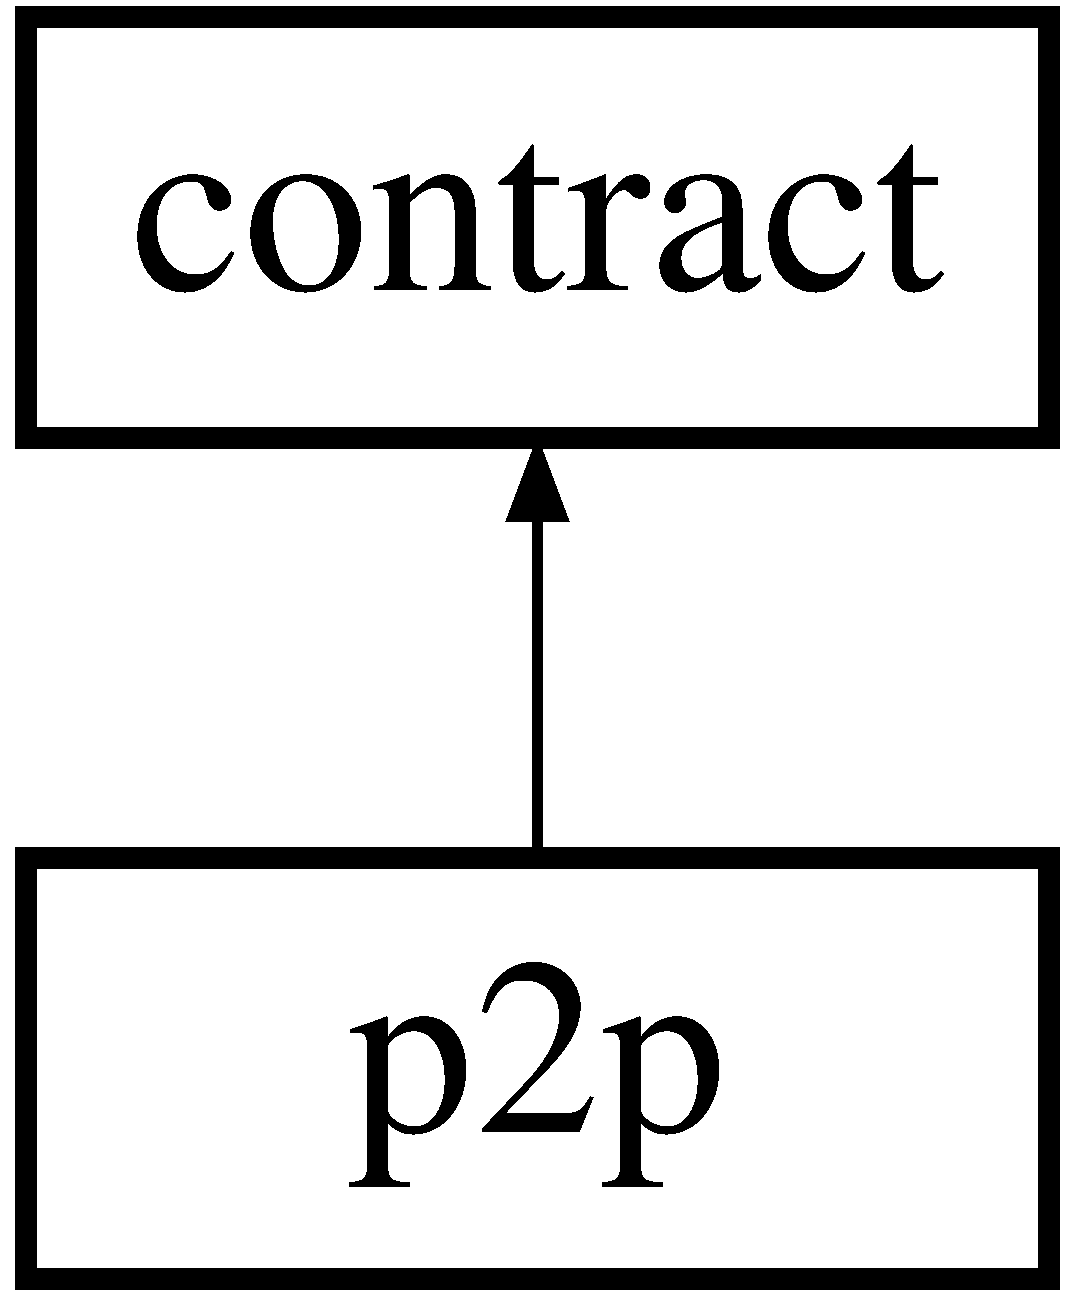
\includegraphics[height=2.000000cm]{classp2p}
\end{center}
\end{figure}
\subsection*{Classes}
\begin{DoxyCompactItemize}
\item 
struct \mbox{\hyperlink{structp2p_1_1balance}{balance}}
\begin{DoxyCompactList}\small\item\em Таблица промежуточного хранения балансов пользователей. \end{DoxyCompactList}\item 
struct \mbox{\hyperlink{structp2p_1_1bbonuses}{bbonuses}}
\begin{DoxyCompactList}\small\item\em Таблица резервов контракта для выплат бонусов в реферальную сеть \end{DoxyCompactList}\item 
struct \mbox{\hyperlink{structp2p_1_1counts}{counts}}
\begin{DoxyCompactList}\small\item\em Таблица счётчиков ордеров \end{DoxyCompactList}\item 
struct \mbox{\hyperlink{structp2p_1_1guests}{guests}}
\begin{DoxyCompactList}\small\item\em Таблица доступа к записям гостей платформы \end{DoxyCompactList}\item 
struct \mbox{\hyperlink{structp2p_1_1orders}{orders}}
\begin{DoxyCompactList}\small\item\em Таблица ордеров \end{DoxyCompactList}\item 
struct \mbox{\hyperlink{structp2p_1_1usdrates}{usdrates}}
\begin{DoxyCompactList}\small\item\em Таблица содержит курсы конвертации к доллару. \end{DoxyCompactList}\item 
struct \mbox{\hyperlink{structp2p_1_1usdrates2}{usdrates2}}
\begin{DoxyCompactList}\small\item\em Таблица расширения usdrates с указанием даты установки первого курса \end{DoxyCompactList}\item 
struct \mbox{\hyperlink{structp2p_1_1vesting}{vesting}}
\begin{DoxyCompactList}\small\item\em Таблица вестинг-\/балансов пользователей \end{DoxyCompactList}\end{DoxyCompactItemize}
\subsection*{Public Types}
\begin{DoxyCompactItemize}
\item 
\mbox{\Hypertarget{classp2p_a562223292a6b99a97d486136b2eb0d9e}\label{classp2p_a562223292a6b99a97d486136b2eb0d9e}} 
typedef eosio\+::multi\+\_\+index$<$\char`\"{}balance\char`\"{}\+\_\+n, \mbox{\hyperlink{structp2p_1_1balance}{balance}}, eosio\+::indexed\+\_\+by$<$ \char`\"{}byconsym\char`\"{}\+\_\+n, eosio\+::const\+\_\+mem\+\_\+fun$<$ \mbox{\hyperlink{structp2p_1_1balance}{balance}}, uint128\+\_\+t, \&balance\+::byconsym $>$ $>$ $>$ {\bfseries balances\+\_\+index}
\item 
\mbox{\Hypertarget{classp2p_a6bef060ed784c193c2a60b397c869c29}\label{classp2p_a6bef060ed784c193c2a60b397c869c29}} 
typedef eosio\+::multi\+\_\+index$<$\char`\"{}counts\char`\"{}\+\_\+n, \mbox{\hyperlink{structp2p_1_1counts}{counts}} $>$ {\bfseries counts\+\_\+index}
\item 
\mbox{\Hypertarget{classp2p_af7e337013ebdcc44b420a6d55d0d385f}\label{classp2p_af7e337013ebdcc44b420a6d55d0d385f}} 
typedef eosio\+::multi\+\_\+index$<$ \char`\"{}orders\char`\"{}\+\_\+n, \mbox{\hyperlink{structp2p_1_1orders}{orders}}, eosio\+::indexed\+\_\+by$<$\char`\"{}bycurrcode\char`\"{}\+\_\+n, eosio\+::const\+\_\+mem\+\_\+fun$<$ \mbox{\hyperlink{structp2p_1_1orders}{orders}}, uint64\+\_\+t, \&\mbox{\hyperlink{structp2p_1_1orders_ab6f05a725122c94d3f2dcfaf24322c47}{orders\+::bycurrcode}} $>$ $>$, eosio\+::indexed\+\_\+by$<$\char`\"{}byparentid\char`\"{}\+\_\+n, eosio\+::const\+\_\+mem\+\_\+fun$<$ \mbox{\hyperlink{structp2p_1_1orders}{orders}}, uint64\+\_\+t, \&\mbox{\hyperlink{structp2p_1_1orders_a2b790da517561e8a593b6c56d63c4cfd}{orders\+::byparentid}} $>$ $>$, eosio\+::indexed\+\_\+by$<$\char`\"{}bytype\char`\"{}\+\_\+n, eosio\+::const\+\_\+mem\+\_\+fun$<$ \mbox{\hyperlink{structp2p_1_1orders}{orders}}, uint64\+\_\+t, \&\mbox{\hyperlink{structp2p_1_1orders_a17505cc3759a5ba5099f490c982535e1}{orders\+::bytype}} $>$ $>$, eosio\+::indexed\+\_\+by$<$\char`\"{}bycreator\char`\"{}\+\_\+n, eosio\+::const\+\_\+mem\+\_\+fun$<$ \mbox{\hyperlink{structp2p_1_1orders}{orders}}, uint64\+\_\+t, \&\mbox{\hyperlink{structp2p_1_1orders_a91b49c417f79ef405982bfe348651a98}{orders\+::bycreator}} $>$ $>$, eosio\+::indexed\+\_\+by$<$\char`\"{}bycurator\char`\"{}\+\_\+n, eosio\+::const\+\_\+mem\+\_\+fun$<$ \mbox{\hyperlink{structp2p_1_1orders}{orders}}, uint64\+\_\+t, \&\mbox{\hyperlink{structp2p_1_1orders_a76fa8b54f391ccd2e29b640d4c0199df}{orders\+::bycurator}} $>$ $>$, eosio\+::indexed\+\_\+by$<$\char`\"{}bystatus\char`\"{}\+\_\+n, eosio\+::const\+\_\+mem\+\_\+fun$<$ \mbox{\hyperlink{structp2p_1_1orders}{orders}}, uint64\+\_\+t, \&\mbox{\hyperlink{structp2p_1_1orders_a31e70a285fb324d4ee07b1b149debff3}{orders\+::bystatus}} $>$ $>$, eosio\+::indexed\+\_\+by$<$\char`\"{}byexpr\char`\"{}\+\_\+n, eosio\+::const\+\_\+mem\+\_\+fun$<$ \mbox{\hyperlink{structp2p_1_1orders}{orders}}, uint64\+\_\+t, \&\mbox{\hyperlink{structp2p_1_1orders_a8cf94dfb0902511c6baae1dd0434dcbf}{orders\+::byexpr}} $>$ $>$, eosio\+::indexed\+\_\+by$<$\char`\"{}bycreated\char`\"{}\+\_\+n, eosio\+::const\+\_\+mem\+\_\+fun$<$ \mbox{\hyperlink{structp2p_1_1orders}{orders}}, uint64\+\_\+t, \&\mbox{\hyperlink{structp2p_1_1orders_a6eab9cb4d0f7b605aef8856aad730fe5}{orders\+::bycreated}} $>$ $>$ $>$ {\bfseries orders\+\_\+index}
\item 
\mbox{\Hypertarget{classp2p_ac0dc7fa780d52c554aea91ab34bb3cfb}\label{classp2p_ac0dc7fa780d52c554aea91ab34bb3cfb}} 
typedef eosio\+::multi\+\_\+index$<$\char`\"{}usdrates\char`\"{}\+\_\+n, \mbox{\hyperlink{structp2p_1_1usdrates}{usdrates}}, eosio\+::indexed\+\_\+by$<$ \char`\"{}byconsym\char`\"{}\+\_\+n, eosio\+::const\+\_\+mem\+\_\+fun$<$ \mbox{\hyperlink{structp2p_1_1usdrates}{usdrates}}, uint128\+\_\+t, \&\mbox{\hyperlink{structp2p_1_1usdrates_a6d13bdd9e62d26ca68146e642e330099}{usdrates\+::byconsym}} $>$ $>$ $>$ {\bfseries usdrates\+\_\+index}
\item 
\mbox{\Hypertarget{classp2p_abbacbe5996794991fcbfb554dae6dc41}\label{classp2p_abbacbe5996794991fcbfb554dae6dc41}} 
typedef eosio\+::multi\+\_\+index$<$\char`\"{}usdrates2\char`\"{}\+\_\+n, \mbox{\hyperlink{structp2p_1_1usdrates2}{usdrates2}} $>$ {\bfseries usdrates2\+\_\+index}
\item 
\mbox{\Hypertarget{classp2p_ad2b234c3e4a379adfeebb42efe3fdb25}\label{classp2p_ad2b234c3e4a379adfeebb42efe3fdb25}} 
typedef eosio\+::multi\+\_\+index$<$\char`\"{}bbonuses\char`\"{}\+\_\+n, \mbox{\hyperlink{structp2p_1_1bbonuses}{bbonuses}} $>$ {\bfseries bbonuses\+\_\+index}
\item 
\mbox{\Hypertarget{classp2p_a9e10c97b92e817371f627c84094dce39}\label{classp2p_a9e10c97b92e817371f627c84094dce39}} 
typedef eosio\+::multi\+\_\+index$<$\char`\"{}vesting\char`\"{}\+\_\+n, \mbox{\hyperlink{structp2p_1_1vesting}{vesting}} $>$ {\bfseries vesting\+\_\+index}
\item 
\mbox{\Hypertarget{classp2p_a08507c2c104ad7e99765afd19d4fdd10}\label{classp2p_a08507c2c104ad7e99765afd19d4fdd10}} 
typedef eosio\+::multi\+\_\+index$<$\char`\"{}guests\char`\"{}\+\_\+n, \mbox{\hyperlink{structp2p_1_1guests}{guests}}, eosio\+::indexed\+\_\+by$<$ \char`\"{}byexpr\char`\"{}\+\_\+n, eosio\+::const\+\_\+mem\+\_\+fun$<$ \mbox{\hyperlink{structp2p_1_1guests}{guests}}, uint64\+\_\+t, \&guests\+::byexpr $>$ $>$, eosio\+::indexed\+\_\+by$<$ \char`\"{}byreg\char`\"{}\+\_\+n, eosio\+::const\+\_\+mem\+\_\+fun$<$ \mbox{\hyperlink{structp2p_1_1guests}{guests}}, uint64\+\_\+t, \&guests\+::byreg $>$ $>$ $>$ {\bfseries guests\+\_\+index}
\end{DoxyCompactItemize}
\subsection*{Public Member Functions}
\begin{DoxyCompactItemize}
\item 
\mbox{\Hypertarget{classp2p_a5dac3e80d9e970fbc86c4fbaf781f894}\label{classp2p_a5dac3e80d9e970fbc86c4fbaf781f894}} 
{\bfseries p2p} (eosio\+::name receiver, eosio\+::name code, eosio\+::datastream$<$ const char $\ast$$>$ ds)
\item 
\mbox{\Hypertarget{classp2p_a1ba9938186b683d21e39ae021d7a0a6f}\label{classp2p_a1ba9938186b683d21e39ae021d7a0a6f}} 
void {\bfseries apply} (uint64\+\_\+t receiver, uint64\+\_\+t code, uint64\+\_\+t action)
\item 
void \mbox{\hyperlink{classp2p_a0b05f55568e9469d33379512b29a116a}{createorder}} (name username, uint64\+\_\+t parent\+\_\+id, name type, eosio\+::name root\+\_\+contract, eosio\+::asset root\+\_\+quantity, eosio\+::name quote\+\_\+type, double quote\+\_\+rate, eosio\+::name quote\+\_\+contract, eosio\+::asset quote\+\_\+quantity, eosio\+::name out\+\_\+type, double out\+\_\+rate, eosio\+::name out\+\_\+contract, eosio\+::asset out\+\_\+quantity, std\+::string details)
\begin{DoxyCompactList}\small\item\em Метод создания ордера \end{DoxyCompactList}\item 
void \mbox{\hyperlink{classp2p_ab7d91c105e22cc794a42cb12d996d0cb}{accept}} (name username, uint64\+\_\+t id, std\+::string details)
\begin{DoxyCompactList}\small\item\em Метод подтверждения факта присутствия и начало сделки \end{DoxyCompactList}\item 
void \mbox{\hyperlink{classp2p_a4562d6493c57589bf2259f119481d39a}{approve}} (name username, uint64\+\_\+t id)
\begin{DoxyCompactList}\small\item\em Метод утверждения завершенного ордера \end{DoxyCompactList}\item 
void \mbox{\hyperlink{classp2p_aa1abaf488133faec3fae6c6c9c9917c2}{confirm}} (name username, uint64\+\_\+t id)
\begin{DoxyCompactList}\small\item\em Метод подтверждения факта платежа \end{DoxyCompactList}\item 
void \mbox{\hyperlink{classp2p_af81f265e37d1f1572a9a5fa17fa99f32}{cancel}} (name username, uint64\+\_\+t id)
\begin{DoxyCompactList}\small\item\em Метод отмены ордера \end{DoxyCompactList}\item 
void \mbox{\hyperlink{classp2p_a4f0c0c376096f7a73b21b39f0dc58d1d}{dispute}} (name username, uint64\+\_\+t id)
\begin{DoxyCompactList}\small\item\em Метод создания спора \end{DoxyCompactList}\item 
void \mbox{\hyperlink{classp2p_a805effb2c6e15ab30e7f36bf13558910}{del}} (name username, uint64\+\_\+t id)
\begin{DoxyCompactList}\small\item\em Метод удаления завершенной сделки из оперативной памяти \end{DoxyCompactList}\item 
void \mbox{\hyperlink{classp2p_a432842119735888f862933882e6a4da6}{setrate}} (eosio\+::name out\+\_\+contract, eosio\+::asset out\+\_\+asset, double rate)
\begin{DoxyCompactList}\small\item\em Метод установки курса обмена к U\+SD. \end{DoxyCompactList}\item 
void \mbox{\hyperlink{classp2p_a6684d814e1a17f87c492e2b394cc1846}{uprate}} (eosio\+::name out\+\_\+contract, eosio\+::asset out\+\_\+asset)
\begin{DoxyCompactList}\small\item\em Метод увеличения курса обмена системного токена \end{DoxyCompactList}\item 
void \mbox{\hyperlink{classp2p_abea413390558d072de45f9ff47217ff8}{delrate}} (uint64\+\_\+t id)
\begin{DoxyCompactList}\small\item\em Метод удаление курса \end{DoxyCompactList}\item 
void \mbox{\hyperlink{classp2p_a6ef3ff3b489159e054195c1d8fbd7092}{delvesting}} (eosio\+::name owner, uint64\+\_\+t id)
\begin{DoxyCompactList}\small\item\em Метод удаление вестинг-\/баланса \end{DoxyCompactList}\item 
void \mbox{\hyperlink{classp2p_a4f3c89b4ae21f54b6e16334e681a7860}{setbrate}} (eosio\+::name host, double distribution\+\_\+rate)
\begin{DoxyCompactList}\small\item\em Метод установки бонусного курса \end{DoxyCompactList}\item 
void \mbox{\hyperlink{classp2p_a2cb80d56fbb68ac3ccc688112d86532a}{refreshsh}} (eosio\+::name owner, uint64\+\_\+t id)
\begin{DoxyCompactList}\small\item\em Метод обновления вестинг-\/баланса. ~\newline
 \end{DoxyCompactList}\item 
void \mbox{\hyperlink{classp2p_adb4fde78468ee3b060717a785febdcc4}{withdrawsh}} (eosio\+::name owner, uint64\+\_\+t id)
\begin{DoxyCompactList}\small\item\em Вывод вестинг-\/баланса \end{DoxyCompactList}\end{DoxyCompactItemize}
\subsection*{Static Public Member Functions}
\begin{DoxyCompactItemize}
\item 
\mbox{\Hypertarget{classp2p_ac36f6042dcb8942679dddbf672684ddc}\label{classp2p_ac36f6042dcb8942679dddbf672684ddc}} 
static void {\bfseries add\+\_\+balance} (eosio\+::name payer, eosio\+::asset quantity, eosio\+::name contract)
\item 
\mbox{\Hypertarget{classp2p_afc44fa7dedaeea9559af5f70445b5218}\label{classp2p_afc44fa7dedaeea9559af5f70445b5218}} 
static void {\bfseries sub\+\_\+balance} (eosio\+::name username, eosio\+::asset quantity, eosio\+::name contract)
\item 
\mbox{\Hypertarget{classp2p_aa6f449f9ebec47b6741ed3497a3b92f9}\label{classp2p_aa6f449f9ebec47b6741ed3497a3b92f9}} 
static void {\bfseries addbbal} (eosio\+::name host, eosio\+::name contract, eosio\+::asset quantity)
\item 
\mbox{\Hypertarget{classp2p_a9bbb48f7000e2ad2c901fe04f3e7f024}\label{classp2p_a9bbb48f7000e2ad2c901fe04f3e7f024}} 
static void {\bfseries subbbal} (eosio\+::name host, eosio\+::name contract, eosio\+::asset quantity)
\item 
\mbox{\Hypertarget{classp2p_a0b427c0584a5dd22a924273d3476dfd7}\label{classp2p_a0b427c0584a5dd22a924273d3476dfd7}} 
static void {\bfseries make\+\_\+vesting\+\_\+action} (eosio\+::name owner, eosio\+::name contract, eosio\+::asset amount)
\item 
\mbox{\Hypertarget{classp2p_ac62758f88566e5dafc0804182f324658}\label{classp2p_ac62758f88566e5dafc0804182f324658}} 
static void {\bfseries check\+\_\+bonuse\+\_\+system} (eosio\+::name creator, eosio\+::name reciever, eosio\+::asset quantity)
\item 
\mbox{\Hypertarget{classp2p_a5a20e06fb911402d5e343389bdf944d4}\label{classp2p_a5a20e06fb911402d5e343389bdf944d4}} 
static void {\bfseries check\+\_\+guest\+\_\+and\+\_\+gift\+\_\+account} (eosio\+::name username, eosio\+::name contract, eosio\+::asset amount)
\item 
\mbox{\Hypertarget{classp2p_a6277838ad086e92577864a4c59ec3e6c}\label{classp2p_a6277838ad086e92577864a4c59ec3e6c}} 
static uint64\+\_\+t {\bfseries get\+\_\+order\+\_\+id} ()
\item 
\mbox{\Hypertarget{classp2p_a4aa15958215b4647e9adc4ed3d53af8c}\label{classp2p_a4aa15958215b4647e9adc4ed3d53af8c}} 
static uint128\+\_\+t {\bfseries combine\+\_\+ids} (const uint64\+\_\+t \&x, const uint64\+\_\+t \&y)
\end{DoxyCompactItemize}
\subsection*{Static Public Attributes}
\begin{DoxyCompactItemize}
\item 
static constexpr eosio\+::name \mbox{\hyperlink{classp2p_ade9426b6e05cdb60d41e808717199b89}{\+\_\+me}} = \char`\"{}p2p\char`\"{}\+\_\+n
\item 
static constexpr eosio\+::name \mbox{\hyperlink{classp2p_aa5528a78186585c3a033d89b6c027a5b}{\+\_\+curator}} = \char`\"{}p2p\char`\"{}\+\_\+n
\item 
static constexpr eosio\+::name \mbox{\hyperlink{classp2p_abaf26be47ba132e33bdadf4a6f65a052}{\+\_\+rater}} = \char`\"{}rater\char`\"{}\+\_\+n
\item 
static constexpr eosio\+::symbol \mbox{\hyperlink{classp2p_afe8d32633b8a87ce35209184d222f6de}{\+\_\+\+S\+YM}} = eosio\+::symbol(eosio\+::symbol\+\_\+code(\char`\"{}N\+BT\char`\"{}), 4)
\item 
static constexpr eosio\+::name \mbox{\hyperlink{classp2p_a582434add36ca36a326bdab9e7c8cb4e}{\+\_\+core}} = \char`\"{}unicore\char`\"{}\+\_\+n
\item 
static const uint64\+\_\+t \mbox{\hyperlink{classp2p_a6a7a6607c93e930cfa3984a8c318942b}{\+\_\+\+P\+E\+R\+C\+E\+N\+T\+S\+\_\+\+P\+E\+R\+\_\+\+M\+O\+N\+TH}} = 42
\item 
static const bool \mbox{\hyperlink{classp2p_a738ddf63d1276c74f28b7d2f51ba1475}{\+\_\+\+E\+N\+A\+B\+L\+E\+\_\+\+G\+R\+O\+W\+HT}} = true
\item 
static const bool \mbox{\hyperlink{classp2p_a817118e4e422393acc35439edb0187af}{\+\_\+\+E\+N\+A\+B\+L\+E\+\_\+\+V\+E\+S\+T\+I\+NG}} = true
\item 
static const uint64\+\_\+t \mbox{\hyperlink{classp2p_af52bcfc4c42cb8a001ab4935d06539c0}{\+\_\+\+V\+E\+S\+T\+I\+N\+G\+\_\+\+S\+E\+C\+O\+N\+DS}} = 15770000
\item 
static constexpr eosio\+::name \mbox{\hyperlink{classp2p_aaf70e52c0f57cc4fa3d9d7fd0e8f0d99}{\+\_\+\+C\+O\+R\+E\+\_\+\+S\+A\+L\+E\+\_\+\+A\+C\+C\+O\+U\+NT}} = \char`\"{}core\char`\"{}\+\_\+n
\item 
static constexpr eosio\+::name \mbox{\hyperlink{classp2p_ad3c9fd465ea37d16657bd9910c631d22}{\+\_\+\+R\+E\+G\+I\+S\+T\+R\+A\+T\+O\+R\+\_\+\+A\+C\+C\+O\+U\+NT}} = \char`\"{}registrator\char`\"{}\+\_\+n
\item 
static const uint64\+\_\+t \mbox{\hyperlink{classp2p_ada18e95b855fa10dc57a33620b4dd51d}{\+\_\+\+G\+I\+F\+T\+\_\+\+A\+C\+C\+O\+U\+N\+T\+\_\+\+F\+R\+O\+M\+\_\+\+A\+M\+O\+U\+NT}} = 100000
\item 
static const uint64\+\_\+t \mbox{\hyperlink{classp2p_a714001f0f556d0db16b3746fa2261ddb}{\+\_\+\+O\+R\+D\+E\+R\+\_\+\+E\+X\+P\+I\+R\+A\+T\+I\+ON}} = 30 $\ast$ 60
\item 
static constexpr double \mbox{\hyperlink{classp2p_a41fd0523f7a4103ea012c69c376d0823}{\+\_\+\+S\+T\+A\+R\+T\+\_\+\+R\+A\+TE}} = 0.\+2
\end{DoxyCompactItemize}


\subsection{Detailed Description}
Начните ознакомление здесь. 

\subsection{Member Function Documentation}
\mbox{\Hypertarget{classp2p_ab7d91c105e22cc794a42cb12d996d0cb}\label{classp2p_ab7d91c105e22cc794a42cb12d996d0cb}} 
\index{p2p@{p2p}!accept@{accept}}
\index{accept@{accept}!p2p@{p2p}}
\subsubsection{\texorpdfstring{accept()}{accept()}}
{\footnotesize\ttfamily void p2p\+::accept (\begin{DoxyParamCaption}\item[{name}]{username,  }\item[{uint64\+\_\+t}]{id,  }\item[{std\+::string}]{details }\end{DoxyParamCaption})}



Метод подтверждения факта присутствия и начало сделки 

A\+U\+TH = username

Реквизиты для оплаты передаются в поле details, если дочерний ордер типа buy. Статус ордера изменяется на process. 
\begin{DoxyParams}[1]{Parameters}
\mbox{\tt in}  & {\em username} & имя пользователя, подтверждающего начало сделки \\
\hline
\mbox{\tt in}  & {\em id} & идентификатор ордера \\
\hline
\mbox{\tt in}  & {\em details} & реквизиты для получения оплаты по сделке \\
\hline
\end{DoxyParams}
\mbox{\Hypertarget{classp2p_a4562d6493c57589bf2259f119481d39a}\label{classp2p_a4562d6493c57589bf2259f119481d39a}} 
\index{p2p@{p2p}!approve@{approve}}
\index{approve@{approve}!p2p@{p2p}}
\subsubsection{\texorpdfstring{approve()}{approve()}}
{\footnotesize\ttfamily void p2p\+::approve (\begin{DoxyParamCaption}\item[{name}]{username,  }\item[{uint64\+\_\+t}]{id }\end{DoxyParamCaption})}



Метод утверждения завершенного ордера 

A\+U\+TH = username

После получения оплаты, пользователь должен вызовать этот метод и утвердить завершение сделки, разблокировав токены для второго участника сделки. Статус ордера изменяется на finish и производится разблокирование токенов для получателя. 
\begin{DoxyParams}[1]{Parameters}
\mbox{\tt in}  & {\em username} & имя аккаунта участника сделки, утверждающего успешное завершение сделки \\
\hline
\mbox{\tt in}  & {\em id} & идентификатор ордера \\
\hline
\end{DoxyParams}
\mbox{\Hypertarget{classp2p_af81f265e37d1f1572a9a5fa17fa99f32}\label{classp2p_af81f265e37d1f1572a9a5fa17fa99f32}} 
\index{p2p@{p2p}!cancel@{cancel}}
\index{cancel@{cancel}!p2p@{p2p}}
\subsubsection{\texorpdfstring{cancel()}{cancel()}}
{\footnotesize\ttfamily void p2p\+::cancel (\begin{DoxyParamCaption}\item[{name}]{username,  }\item[{uint64\+\_\+t}]{id }\end{DoxyParamCaption})}



Метод отмены ордера 

A\+U\+TH = username

Отменяет ордер и удаляет его из оперативной памяти, разблокируя средства согласну типу ордера. 
\begin{DoxyParams}[1]{Parameters}
\mbox{\tt in}  & {\em username} & имя аккаунта участника сделки, производящего отмену ордера. \\
\hline
\mbox{\tt in}  & {\em id} & идентификатор ордера \\
\hline
\end{DoxyParams}
\mbox{\Hypertarget{classp2p_aa1abaf488133faec3fae6c6c9c9917c2}\label{classp2p_aa1abaf488133faec3fae6c6c9c9917c2}} 
\index{p2p@{p2p}!confirm@{confirm}}
\index{confirm@{confirm}!p2p@{p2p}}
\subsubsection{\texorpdfstring{confirm()}{confirm()}}
{\footnotesize\ttfamily void p2p\+::confirm (\begin{DoxyParamCaption}\item[{name}]{username,  }\item[{uint64\+\_\+t}]{id }\end{DoxyParamCaption})}



Метод подтверждения факта платежа 

A\+U\+TH = username

После совершения оплаты на реквизиты, участник сделки должен подтвердить этот факт вызовом этого метода. Статус ордера изменяется на payed. 
\begin{DoxyParams}[1]{Parameters}
\mbox{\tt in}  & {\em username} & имя аккаунта участника сделки, утверждающего факт совершения оплаты на реквизиты \\
\hline
\mbox{\tt in}  & {\em id} & идентификатор ордера \\
\hline
\end{DoxyParams}
\mbox{\Hypertarget{classp2p_a0b05f55568e9469d33379512b29a116a}\label{classp2p_a0b05f55568e9469d33379512b29a116a}} 
\index{p2p@{p2p}!createorder@{createorder}}
\index{createorder@{createorder}!p2p@{p2p}}
\subsubsection{\texorpdfstring{createorder()}{createorder()}}
{\footnotesize\ttfamily void p2p\+::createorder (\begin{DoxyParamCaption}\item[{name}]{username,  }\item[{uint64\+\_\+t}]{parent\+\_\+id,  }\item[{name}]{type,  }\item[{eosio\+::name}]{root\+\_\+contract,  }\item[{eosio\+::asset}]{root\+\_\+quantity,  }\item[{eosio\+::name}]{quote\+\_\+type,  }\item[{double}]{quote\+\_\+rate,  }\item[{eosio\+::name}]{quote\+\_\+contract,  }\item[{eosio\+::asset}]{quote\+\_\+quantity,  }\item[{eosio\+::name}]{out\+\_\+type,  }\item[{double}]{out\+\_\+rate,  }\item[{eosio\+::name}]{out\+\_\+contract,  }\item[{eosio\+::asset}]{out\+\_\+quantity,  }\item[{std\+::string}]{details }\end{DoxyParamCaption})}



Метод создания ордера 

A\+U\+TH = username

Используя метод, пользователь создаёт ордер для обмена.


\begin{DoxyParams}[1]{Parameters}
\mbox{\tt in}  & {\em username} & Имя пользователя, инициирующего обмен \\
\hline
\mbox{\tt in}  & {\em parent\+\_\+id} & Опциональный идентификатор родительской сделки, с которой происходит обмен. Если не установлен -\/ ордер ожидает появление дочерних ордеров в статусе waiting, предлагающих обмен. \\
\hline
\mbox{\tt in}  & {\em type} & Тип ордера buy / sell \\
\hline
\mbox{\tt in}  & {\em root\+\_\+contract} & Имя контракта токена обмена \\
\hline
\mbox{\tt in}  & {\em root\+\_\+quantity} & Количество токенов на обмене \\
\hline
\mbox{\tt in}  & {\em quote\+\_\+type} & Тип опорной валюты, сейчас используем только тип external \\
\hline
\mbox{\tt in}  & {\em quote\+\_\+rate} & Опорный курс обмена \\
\hline
\mbox{\tt in}  & {\em quote\+\_\+contract} & Опорный контракт обмена, сейчас используем только \char`\"{}\char`\"{} \\
\hline
\mbox{\tt in}  & {\em quote\+\_\+quantity} & Количество опорной валюты на обмене, измеряемой в U\+SD \\
\hline
\mbox{\tt in}  & {\em out\+\_\+type} & Тип валюты выхода (сейчас любой) \\
\hline
\mbox{\tt in}  & {\em out\+\_\+rate} & Курс валюты выхода \\
\hline
\mbox{\tt in}  & {\em out\+\_\+contract} & Контракт валюты выхода (сейчас только \char`\"{}\char`\"{}) \\
\hline
\mbox{\tt in}  & {\em out\+\_\+quantity} & Количество валюты выхода \\
\hline
\mbox{\tt in}  & {\em details} & Реквизиты для получения платежа, используются если тип нового ордера = buy \\
\hline
\end{DoxyParams}
\mbox{\Hypertarget{classp2p_a805effb2c6e15ab30e7f36bf13558910}\label{classp2p_a805effb2c6e15ab30e7f36bf13558910}} 
\index{p2p@{p2p}!del@{del}}
\index{del@{del}!p2p@{p2p}}
\subsubsection{\texorpdfstring{del()}{del()}}
{\footnotesize\ttfamily void p2p\+::del (\begin{DoxyParamCaption}\item[{name}]{username,  }\item[{uint64\+\_\+t}]{id }\end{DoxyParamCaption})}



Метод удаления завершенной сделки из оперативной памяти 

A\+U\+TH = username

Очищает завершенную сделку из оперативной памяти операционной системы. 
\begin{DoxyParams}[1]{Parameters}
\mbox{\tt in}  & {\em username} & имя аккаунта, производящего очищение \\
\hline
\mbox{\tt in}  & {\em id} & идентификатор ордера \\
\hline
\end{DoxyParams}
\mbox{\Hypertarget{classp2p_abea413390558d072de45f9ff47217ff8}\label{classp2p_abea413390558d072de45f9ff47217ff8}} 
\index{p2p@{p2p}!delrate@{delrate}}
\index{delrate@{delrate}!p2p@{p2p}}
\subsubsection{\texorpdfstring{delrate()}{delrate()}}
{\footnotesize\ttfamily void p2p\+::delrate (\begin{DoxyParamCaption}\item[{uint64\+\_\+t}]{id }\end{DoxyParamCaption})}



Метод удаление курса 

A\+U\+TH = eosio

Используется администратором для удаления курса из таблицы курсов 
\begin{DoxyParams}[1]{Parameters}
\mbox{\tt in}  & {\em id} & идентификатор курса \\
\hline
\end{DoxyParams}
\mbox{\Hypertarget{classp2p_a6ef3ff3b489159e054195c1d8fbd7092}\label{classp2p_a6ef3ff3b489159e054195c1d8fbd7092}} 
\index{p2p@{p2p}!delvesting@{delvesting}}
\index{delvesting@{delvesting}!p2p@{p2p}}
\subsubsection{\texorpdfstring{delvesting()}{delvesting()}}
{\footnotesize\ttfamily void p2p\+::delvesting (\begin{DoxyParamCaption}\item[{eosio\+::name}]{owner,  }\item[{uint64\+\_\+t}]{id }\end{DoxyParamCaption})}



Метод удаление вестинг-\/баланса 

A\+U\+TH = \mbox{\hyperlink{classp2p}{p2p}}

Используется администратором для удаления ошибочного начисления вестинг-\/баланса 
\begin{DoxyParams}[1]{Parameters}
\mbox{\tt in}  & {\em owner} & имя аккаунта владельца вестинг-\/баланса \\
\hline
\mbox{\tt in}  & {\em id} & идентификатор вестинг-\/баланса \\
\hline
\end{DoxyParams}
\mbox{\Hypertarget{classp2p_a4f0c0c376096f7a73b21b39f0dc58d1d}\label{classp2p_a4f0c0c376096f7a73b21b39f0dc58d1d}} 
\index{p2p@{p2p}!dispute@{dispute}}
\index{dispute@{dispute}!p2p@{p2p}}
\subsubsection{\texorpdfstring{dispute()}{dispute()}}
{\footnotesize\ttfamily void p2p\+::dispute (\begin{DoxyParamCaption}\item[{name}]{username,  }\item[{uint64\+\_\+t}]{id }\end{DoxyParamCaption})}



Метод создания спора 

A\+U\+TH = username

Перевод сделку в статус спора, блокируя вывод средств до его разрешения. Только сделка в статусе payed может быть переведена в статус спора. 
\begin{DoxyParams}[1]{Parameters}
\mbox{\tt in}  & {\em username} & имя аккаунта участника сделки, инициирующего спор \\
\hline
\mbox{\tt in}  & {\em id} & идентификатор ордера \\
\hline
\end{DoxyParams}
\mbox{\Hypertarget{classp2p_a2cb80d56fbb68ac3ccc688112d86532a}\label{classp2p_a2cb80d56fbb68ac3ccc688112d86532a}} 
\index{p2p@{p2p}!refreshsh@{refreshsh}}
\index{refreshsh@{refreshsh}!p2p@{p2p}}
\subsubsection{\texorpdfstring{refreshsh()}{refreshsh()}}
{\footnotesize\ttfamily void p2p\+::refreshsh (\begin{DoxyParamCaption}\item[{eosio\+::name}]{owner,  }\item[{uint64\+\_\+t}]{id }\end{DoxyParamCaption})}



Метод обновления вестинг-\/баланса. ~\newline
 

A\+U\+TH = owner

Обновляет вестинг-\/баланс до доступного остатка. 
\begin{DoxyParams}[1]{Parameters}
\mbox{\tt in}  & {\em owner} & имя аккаунта владельца вестинг-\/баланса \\
\hline
\mbox{\tt in}  & {\em id} & идентификатор вестинг-\/баланса \\
\hline
\end{DoxyParams}
\mbox{\Hypertarget{classp2p_a4f3c89b4ae21f54b6e16334e681a7860}\label{classp2p_a4f3c89b4ae21f54b6e16334e681a7860}} 
\index{p2p@{p2p}!setbrate@{setbrate}}
\index{setbrate@{setbrate}!p2p@{p2p}}
\subsubsection{\texorpdfstring{setbrate()}{setbrate()}}
{\footnotesize\ttfamily void p2p\+::setbrate (\begin{DoxyParamCaption}\item[{eosio\+::name}]{host,  }\item[{double}]{distribution\+\_\+rate }\end{DoxyParamCaption})}



Метод установки бонусного курса 

A\+U\+TH = host

Вызывается владельцем бонусного баланса в контракте для подключения распределения на партнёрскую сеть покупателя.


\begin{DoxyParams}[1]{Parameters}
\mbox{\tt in}  & {\em host} & The host \\
\hline
\mbox{\tt in}  & {\em distribution\+\_\+rate} & The distribution rate \\
\hline
\end{DoxyParams}
\mbox{\Hypertarget{classp2p_a432842119735888f862933882e6a4da6}\label{classp2p_a432842119735888f862933882e6a4da6}} 
\index{p2p@{p2p}!setrate@{setrate}}
\index{setrate@{setrate}!p2p@{p2p}}
\subsubsection{\texorpdfstring{setrate()}{setrate()}}
{\footnotesize\ttfamily void p2p\+::setrate (\begin{DoxyParamCaption}\item[{eosio\+::name}]{out\+\_\+contract,  }\item[{eosio\+::asset}]{out\+\_\+asset,  }\item[{double}]{rate }\end{DoxyParamCaption})}



Метод установки курса обмена к U\+SD. 

A\+U\+TH = \+\_\+rater $\vert$ \+\_\+me

Устанавливает в таблицу usdrates новый актуальный курс от поставщика. 
\begin{DoxyParams}[1]{Parameters}
\mbox{\tt in}  & {\em out\+\_\+contract} & имя контракта выхода (обычно \char`\"{}\char`\"{}) \\
\hline
\mbox{\tt in}  & {\em out\+\_\+asset} & токен выхода с точностью и символом \\
\hline
\mbox{\tt in}  & {\em rate} & курс обмена к U\+SD \\
\hline
\end{DoxyParams}
\mbox{\Hypertarget{classp2p_a6684d814e1a17f87c492e2b394cc1846}\label{classp2p_a6684d814e1a17f87c492e2b394cc1846}} 
\index{p2p@{p2p}!uprate@{uprate}}
\index{uprate@{uprate}!p2p@{p2p}}
\subsubsection{\texorpdfstring{uprate()}{uprate()}}
{\footnotesize\ttfamily void p2p\+::uprate (\begin{DoxyParamCaption}\item[{eosio\+::name}]{out\+\_\+contract,  }\item[{eosio\+::asset}]{out\+\_\+asset }\end{DoxyParamCaption})}



Метод увеличения курса обмена системного токена 

A\+U\+TH = eosio

Периодически вызывается системным контрактом и увеличивает курс обмена системного токена согласно темпу роста в \+\_\+\+P\+E\+R\+C\+E\+N\+T\+S\+\_\+\+P\+E\+R\+\_\+\+M\+O\+N\+TH. 
\begin{DoxyParams}[1]{Parameters}
\mbox{\tt in}  & {\em out\+\_\+contract} & имя контракта выхода (обычно \char`\"{}eosio.\+token\char`\"{}) \\
\hline
\mbox{\tt in}  & {\em out\+\_\+asset} & токен выхода с точностью и символом (обычно равен \+\_\+\+S\+YM) \\
\hline
\end{DoxyParams}
\mbox{\Hypertarget{classp2p_adb4fde78468ee3b060717a785febdcc4}\label{classp2p_adb4fde78468ee3b060717a785febdcc4}} 
\index{p2p@{p2p}!withdrawsh@{withdrawsh}}
\index{withdrawsh@{withdrawsh}!p2p@{p2p}}
\subsubsection{\texorpdfstring{withdrawsh()}{withdrawsh()}}
{\footnotesize\ttfamily void p2p\+::withdrawsh (\begin{DoxyParamCaption}\item[{eosio\+::name}]{owner,  }\item[{uint64\+\_\+t}]{id }\end{DoxyParamCaption})}



Вывод вестинг-\/баланса 

A\+U\+TH = owner

Обеспечивает вывод доступных средств из вестинг-\/баланса. 
\begin{DoxyParams}[1]{Parameters}
\mbox{\tt in}  & {\em owner} & имя аккаунта владельца вестинг-\/баланса \\
\hline
\mbox{\tt in}  & {\em id} & идентификатор вестинг-\/баланса \\
\hline
\end{DoxyParams}


\subsection{Member Data Documentation}
\mbox{\Hypertarget{classp2p_a582434add36ca36a326bdab9e7c8cb4e}\label{classp2p_a582434add36ca36a326bdab9e7c8cb4e}} 
\index{p2p@{p2p}!\+\_\+core@{\+\_\+core}}
\index{\+\_\+core@{\+\_\+core}!p2p@{p2p}}
\subsubsection{\texorpdfstring{\+\_\+core}{\_core}}
{\footnotesize\ttfamily constexpr eosio\+::name p2p\+::\+\_\+core = \char`\"{}unicore\char`\"{}\+\_\+n\hspace{0.3cm}{\ttfamily [static]}}

имя аккаунта распределения реферальных бонусов в сеть \mbox{\Hypertarget{classp2p_aaf70e52c0f57cc4fa3d9d7fd0e8f0d99}\label{classp2p_aaf70e52c0f57cc4fa3d9d7fd0e8f0d99}} 
\index{p2p@{p2p}!\+\_\+\+C\+O\+R\+E\+\_\+\+S\+A\+L\+E\+\_\+\+A\+C\+C\+O\+U\+NT@{\+\_\+\+C\+O\+R\+E\+\_\+\+S\+A\+L\+E\+\_\+\+A\+C\+C\+O\+U\+NT}}
\index{\+\_\+\+C\+O\+R\+E\+\_\+\+S\+A\+L\+E\+\_\+\+A\+C\+C\+O\+U\+NT@{\+\_\+\+C\+O\+R\+E\+\_\+\+S\+A\+L\+E\+\_\+\+A\+C\+C\+O\+U\+NT}!p2p@{p2p}}
\subsubsection{\texorpdfstring{\+\_\+\+C\+O\+R\+E\+\_\+\+S\+A\+L\+E\+\_\+\+A\+C\+C\+O\+U\+NT}{\_CORE\_SALE\_ACCOUNT}}
{\footnotesize\ttfamily constexpr eosio\+::name p2p\+::\+\_\+\+C\+O\+R\+E\+\_\+\+S\+A\+L\+E\+\_\+\+A\+C\+C\+O\+U\+NT = \char`\"{}core\char`\"{}\+\_\+n\hspace{0.3cm}{\ttfamily [static]}}

аккаунт системного продавца токенов, в сделке к которым срабатывает вестинг \mbox{\Hypertarget{classp2p_aa5528a78186585c3a033d89b6c027a5b}\label{classp2p_aa5528a78186585c3a033d89b6c027a5b}} 
\index{p2p@{p2p}!\+\_\+curator@{\+\_\+curator}}
\index{\+\_\+curator@{\+\_\+curator}!p2p@{p2p}}
\subsubsection{\texorpdfstring{\+\_\+curator}{\_curator}}
{\footnotesize\ttfamily constexpr eosio\+::name p2p\+::\+\_\+curator = \char`\"{}p2p\char`\"{}\+\_\+n\hspace{0.3cm}{\ttfamily [static]}}

дефолтное имя аккаунта куратора всех сделок \mbox{\Hypertarget{classp2p_a738ddf63d1276c74f28b7d2f51ba1475}\label{classp2p_a738ddf63d1276c74f28b7d2f51ba1475}} 
\index{p2p@{p2p}!\+\_\+\+E\+N\+A\+B\+L\+E\+\_\+\+G\+R\+O\+W\+HT@{\+\_\+\+E\+N\+A\+B\+L\+E\+\_\+\+G\+R\+O\+W\+HT}}
\index{\+\_\+\+E\+N\+A\+B\+L\+E\+\_\+\+G\+R\+O\+W\+HT@{\+\_\+\+E\+N\+A\+B\+L\+E\+\_\+\+G\+R\+O\+W\+HT}!p2p@{p2p}}
\subsubsection{\texorpdfstring{\+\_\+\+E\+N\+A\+B\+L\+E\+\_\+\+G\+R\+O\+W\+HT}{\_ENABLE\_GROWHT}}
{\footnotesize\ttfamily const bool p2p\+::\+\_\+\+E\+N\+A\+B\+L\+E\+\_\+\+G\+R\+O\+W\+HT = true\hspace{0.3cm}{\ttfamily [static]}}

флаг подключения автоматического роста курса, допускающего вызов метода uprate от системного контракта eosio \mbox{\Hypertarget{classp2p_a817118e4e422393acc35439edb0187af}\label{classp2p_a817118e4e422393acc35439edb0187af}} 
\index{p2p@{p2p}!\+\_\+\+E\+N\+A\+B\+L\+E\+\_\+\+V\+E\+S\+T\+I\+NG@{\+\_\+\+E\+N\+A\+B\+L\+E\+\_\+\+V\+E\+S\+T\+I\+NG}}
\index{\+\_\+\+E\+N\+A\+B\+L\+E\+\_\+\+V\+E\+S\+T\+I\+NG@{\+\_\+\+E\+N\+A\+B\+L\+E\+\_\+\+V\+E\+S\+T\+I\+NG}!p2p@{p2p}}
\subsubsection{\texorpdfstring{\+\_\+\+E\+N\+A\+B\+L\+E\+\_\+\+V\+E\+S\+T\+I\+NG}{\_ENABLE\_VESTING}}
{\footnotesize\ttfamily const bool p2p\+::\+\_\+\+E\+N\+A\+B\+L\+E\+\_\+\+V\+E\+S\+T\+I\+NG = true\hspace{0.3cm}{\ttfamily [static]}}

флаг подключения режима вестинга для совершенных покупок у аккаунта \+\_\+\+C\+O\+R\+E\+\_\+\+S\+A\+L\+E\+\_\+\+A\+C\+C\+O\+U\+NT \mbox{\Hypertarget{classp2p_ada18e95b855fa10dc57a33620b4dd51d}\label{classp2p_ada18e95b855fa10dc57a33620b4dd51d}} 
\index{p2p@{p2p}!\+\_\+\+G\+I\+F\+T\+\_\+\+A\+C\+C\+O\+U\+N\+T\+\_\+\+F\+R\+O\+M\+\_\+\+A\+M\+O\+U\+NT@{\+\_\+\+G\+I\+F\+T\+\_\+\+A\+C\+C\+O\+U\+N\+T\+\_\+\+F\+R\+O\+M\+\_\+\+A\+M\+O\+U\+NT}}
\index{\+\_\+\+G\+I\+F\+T\+\_\+\+A\+C\+C\+O\+U\+N\+T\+\_\+\+F\+R\+O\+M\+\_\+\+A\+M\+O\+U\+NT@{\+\_\+\+G\+I\+F\+T\+\_\+\+A\+C\+C\+O\+U\+N\+T\+\_\+\+F\+R\+O\+M\+\_\+\+A\+M\+O\+U\+NT}!p2p@{p2p}}
\subsubsection{\texorpdfstring{\+\_\+\+G\+I\+F\+T\+\_\+\+A\+C\+C\+O\+U\+N\+T\+\_\+\+F\+R\+O\+M\+\_\+\+A\+M\+O\+U\+NT}{\_GIFT\_ACCOUNT\_FROM\_AMOUNT}}
{\footnotesize\ttfamily const uint64\+\_\+t p2p\+::\+\_\+\+G\+I\+F\+T\+\_\+\+A\+C\+C\+O\+U\+N\+T\+\_\+\+F\+R\+O\+M\+\_\+\+A\+M\+O\+U\+NT = 100000\hspace{0.3cm}{\ttfamily [static]}}

подарок в виде аккаунта партнера осуществляется, если гость совершает покупку на сумму более, чем указано здесь (с учётом точности) \mbox{\Hypertarget{classp2p_ade9426b6e05cdb60d41e808717199b89}\label{classp2p_ade9426b6e05cdb60d41e808717199b89}} 
\index{p2p@{p2p}!\+\_\+me@{\+\_\+me}}
\index{\+\_\+me@{\+\_\+me}!p2p@{p2p}}
\subsubsection{\texorpdfstring{\+\_\+me}{\_me}}
{\footnotesize\ttfamily constexpr eosio\+::name p2p\+::\+\_\+me = \char`\"{}p2p\char`\"{}\+\_\+n\hspace{0.3cm}{\ttfamily [static]}}

собственное имя аккаунта контракта \mbox{\Hypertarget{classp2p_a714001f0f556d0db16b3746fa2261ddb}\label{classp2p_a714001f0f556d0db16b3746fa2261ddb}} 
\index{p2p@{p2p}!\+\_\+\+O\+R\+D\+E\+R\+\_\+\+E\+X\+P\+I\+R\+A\+T\+I\+ON@{\+\_\+\+O\+R\+D\+E\+R\+\_\+\+E\+X\+P\+I\+R\+A\+T\+I\+ON}}
\index{\+\_\+\+O\+R\+D\+E\+R\+\_\+\+E\+X\+P\+I\+R\+A\+T\+I\+ON@{\+\_\+\+O\+R\+D\+E\+R\+\_\+\+E\+X\+P\+I\+R\+A\+T\+I\+ON}!p2p@{p2p}}
\subsubsection{\texorpdfstring{\+\_\+\+O\+R\+D\+E\+R\+\_\+\+E\+X\+P\+I\+R\+A\+T\+I\+ON}{\_ORDER\_EXPIRATION}}
{\footnotesize\ttfamily const uint64\+\_\+t p2p\+::\+\_\+\+O\+R\+D\+E\+R\+\_\+\+E\+X\+P\+I\+R\+A\+T\+I\+ON = 30 $\ast$ 60\hspace{0.3cm}{\ttfamily [static]}}

время до истечения срока давности ордера \mbox{\Hypertarget{classp2p_a6a7a6607c93e930cfa3984a8c318942b}\label{classp2p_a6a7a6607c93e930cfa3984a8c318942b}} 
\index{p2p@{p2p}!\+\_\+\+P\+E\+R\+C\+E\+N\+T\+S\+\_\+\+P\+E\+R\+\_\+\+M\+O\+N\+TH@{\+\_\+\+P\+E\+R\+C\+E\+N\+T\+S\+\_\+\+P\+E\+R\+\_\+\+M\+O\+N\+TH}}
\index{\+\_\+\+P\+E\+R\+C\+E\+N\+T\+S\+\_\+\+P\+E\+R\+\_\+\+M\+O\+N\+TH@{\+\_\+\+P\+E\+R\+C\+E\+N\+T\+S\+\_\+\+P\+E\+R\+\_\+\+M\+O\+N\+TH}!p2p@{p2p}}
\subsubsection{\texorpdfstring{\+\_\+\+P\+E\+R\+C\+E\+N\+T\+S\+\_\+\+P\+E\+R\+\_\+\+M\+O\+N\+TH}{\_PERCENTS\_PER\_MONTH}}
{\footnotesize\ttfamily const uint64\+\_\+t p2p\+::\+\_\+\+P\+E\+R\+C\+E\+N\+T\+S\+\_\+\+P\+E\+R\+\_\+\+M\+O\+N\+TH = 42\hspace{0.3cm}{\ttfamily [static]}}

если рост курса системного токена подключен, то растёт с указанной здесь скоростью \mbox{\Hypertarget{classp2p_abaf26be47ba132e33bdadf4a6f65a052}\label{classp2p_abaf26be47ba132e33bdadf4a6f65a052}} 
\index{p2p@{p2p}!\+\_\+rater@{\+\_\+rater}}
\index{\+\_\+rater@{\+\_\+rater}!p2p@{p2p}}
\subsubsection{\texorpdfstring{\+\_\+rater}{\_rater}}
{\footnotesize\ttfamily constexpr eosio\+::name p2p\+::\+\_\+rater = \char`\"{}rater\char`\"{}\+\_\+n\hspace{0.3cm}{\ttfamily [static]}}

имя аккаунта поставщика курсов \mbox{\Hypertarget{classp2p_ad3c9fd465ea37d16657bd9910c631d22}\label{classp2p_ad3c9fd465ea37d16657bd9910c631d22}} 
\index{p2p@{p2p}!\+\_\+\+R\+E\+G\+I\+S\+T\+R\+A\+T\+O\+R\+\_\+\+A\+C\+C\+O\+U\+NT@{\+\_\+\+R\+E\+G\+I\+S\+T\+R\+A\+T\+O\+R\+\_\+\+A\+C\+C\+O\+U\+NT}}
\index{\+\_\+\+R\+E\+G\+I\+S\+T\+R\+A\+T\+O\+R\+\_\+\+A\+C\+C\+O\+U\+NT@{\+\_\+\+R\+E\+G\+I\+S\+T\+R\+A\+T\+O\+R\+\_\+\+A\+C\+C\+O\+U\+NT}!p2p@{p2p}}
\subsubsection{\texorpdfstring{\+\_\+\+R\+E\+G\+I\+S\+T\+R\+A\+T\+O\+R\+\_\+\+A\+C\+C\+O\+U\+NT}{\_REGISTRATOR\_ACCOUNT}}
{\footnotesize\ttfamily constexpr eosio\+::name p2p\+::\+\_\+\+R\+E\+G\+I\+S\+T\+R\+A\+T\+O\+R\+\_\+\+A\+C\+C\+O\+U\+NT = \char`\"{}registrator\char`\"{}\+\_\+n\hspace{0.3cm}{\ttfamily [static]}}

аккаунт контракта регистратора, хранящего таблицу с гостями для подарочного выкупа \mbox{\Hypertarget{classp2p_a41fd0523f7a4103ea012c69c376d0823}\label{classp2p_a41fd0523f7a4103ea012c69c376d0823}} 
\index{p2p@{p2p}!\+\_\+\+S\+T\+A\+R\+T\+\_\+\+R\+A\+TE@{\+\_\+\+S\+T\+A\+R\+T\+\_\+\+R\+A\+TE}}
\index{\+\_\+\+S\+T\+A\+R\+T\+\_\+\+R\+A\+TE@{\+\_\+\+S\+T\+A\+R\+T\+\_\+\+R\+A\+TE}!p2p@{p2p}}
\subsubsection{\texorpdfstring{\+\_\+\+S\+T\+A\+R\+T\+\_\+\+R\+A\+TE}{\_START\_RATE}}
{\footnotesize\ttfamily constexpr double p2p\+::\+\_\+\+S\+T\+A\+R\+T\+\_\+\+R\+A\+TE = 0.\+2\hspace{0.3cm}{\ttfamily [static]}}

начальный курс старта роста системного токена относительно U\+SD \mbox{\Hypertarget{classp2p_afe8d32633b8a87ce35209184d222f6de}\label{classp2p_afe8d32633b8a87ce35209184d222f6de}} 
\index{p2p@{p2p}!\+\_\+\+S\+YM@{\+\_\+\+S\+YM}}
\index{\+\_\+\+S\+YM@{\+\_\+\+S\+YM}!p2p@{p2p}}
\subsubsection{\texorpdfstring{\+\_\+\+S\+YM}{\_SYM}}
{\footnotesize\ttfamily constexpr eosio\+::symbol p2p\+::\+\_\+\+S\+YM = eosio\+::symbol(eosio\+::symbol\+\_\+code(\char`\"{}N\+BT\char`\"{}), 4)\hspace{0.3cm}{\ttfamily [static]}}

системный токен \mbox{\Hypertarget{classp2p_af52bcfc4c42cb8a001ab4935d06539c0}\label{classp2p_af52bcfc4c42cb8a001ab4935d06539c0}} 
\index{p2p@{p2p}!\+\_\+\+V\+E\+S\+T\+I\+N\+G\+\_\+\+S\+E\+C\+O\+N\+DS@{\+\_\+\+V\+E\+S\+T\+I\+N\+G\+\_\+\+S\+E\+C\+O\+N\+DS}}
\index{\+\_\+\+V\+E\+S\+T\+I\+N\+G\+\_\+\+S\+E\+C\+O\+N\+DS@{\+\_\+\+V\+E\+S\+T\+I\+N\+G\+\_\+\+S\+E\+C\+O\+N\+DS}!p2p@{p2p}}
\subsubsection{\texorpdfstring{\+\_\+\+V\+E\+S\+T\+I\+N\+G\+\_\+\+S\+E\+C\+O\+N\+DS}{\_VESTING\_SECONDS}}
{\footnotesize\ttfamily const uint64\+\_\+t p2p\+::\+\_\+\+V\+E\+S\+T\+I\+N\+G\+\_\+\+S\+E\+C\+O\+N\+DS = 15770000\hspace{0.3cm}{\ttfamily [static]}}

продолжительность вестинга в секундах 

The documentation for this class was generated from the following files\+:\begin{DoxyCompactItemize}
\item 
p2p.\+hpp\item 
p2p.\+cpp\end{DoxyCompactItemize}

\hypertarget{structp2p_1_1usdrates}{}\section{p2p\+:\+:usdrates Struct Reference}
\label{structp2p_1_1usdrates}\index{p2p\+::usdrates@{p2p\+::usdrates}}


Таблица содержит курсы конвертации к доллару.  




{\ttfamily \#include $<$p2p.\+hpp$>$}

\subsection*{Public Member Functions}
\begin{DoxyCompactItemize}
\item 
uint64\+\_\+t \mbox{\hyperlink{structp2p_1_1usdrates_a8bdf953b105c26b52b6fe3be2b910925}{primary\+\_\+key}} () const
\item 
uint128\+\_\+t \mbox{\hyperlink{structp2p_1_1usdrates_a6d13bdd9e62d26ca68146e642e330099}{byconsym}} () const
\end{DoxyCompactItemize}
\subsection*{Public Attributes}
\begin{DoxyCompactItemize}
\item 
uint64\+\_\+t \mbox{\hyperlink{structp2p_1_1usdrates_a5f755d95b0efa7942636fddfae33db2f}{id}}
\item 
eosio\+::name \mbox{\hyperlink{structp2p_1_1usdrates_a6e1aa8746a552939956d3aa3e93782d9}{out\+\_\+contract}}
\item 
eosio\+::asset \mbox{\hyperlink{structp2p_1_1usdrates_ac6ba77785a025d183b2378d5b1bb7f69}{out\+\_\+asset}}
\item 
double \mbox{\hyperlink{structp2p_1_1usdrates_a4a0439519abb54675759686a1b5fe43a}{rate}}
\item 
eosio\+::time\+\_\+point\+\_\+sec \mbox{\hyperlink{structp2p_1_1usdrates_a79bb6e9971e40371c8003013887bf294}{updated\+\_\+at}}
\end{DoxyCompactItemize}


\subsection{Detailed Description}
Таблица содержит курсы конвертации к доллару. 

C\+O\+N\+T\+R\+A\+CT = \+\_\+me, S\+C\+O\+PE = \+\_\+me, T\+A\+B\+LE = usdrates

Курсы обновляются аккаунтом rater методом setrate или системным контрактом eosio методом uprate. 

\subsection{Member Function Documentation}
\mbox{\Hypertarget{structp2p_1_1usdrates_a6d13bdd9e62d26ca68146e642e330099}\label{structp2p_1_1usdrates_a6d13bdd9e62d26ca68146e642e330099}} 
\index{p2p\+::usdrates@{p2p\+::usdrates}!byconsym@{byconsym}}
\index{byconsym@{byconsym}!p2p\+::usdrates@{p2p\+::usdrates}}
\subsubsection{\texorpdfstring{byconsym()}{byconsym()}}
{\footnotesize\ttfamily uint128\+\_\+t p2p\+::usdrates\+::byconsym (\begin{DoxyParamCaption}{ }\end{DoxyParamCaption}) const\hspace{0.3cm}{\ttfamily [inline]}}

(out\+\_\+contract, out\+\_\+asset.\+symbol) -\/ комбинированный secondary\+\_\+key для получения курса по имени выходного контракта и символу \mbox{\Hypertarget{structp2p_1_1usdrates_a8bdf953b105c26b52b6fe3be2b910925}\label{structp2p_1_1usdrates_a8bdf953b105c26b52b6fe3be2b910925}} 
\index{p2p\+::usdrates@{p2p\+::usdrates}!primary\+\_\+key@{primary\+\_\+key}}
\index{primary\+\_\+key@{primary\+\_\+key}!p2p\+::usdrates@{p2p\+::usdrates}}
\subsubsection{\texorpdfstring{primary\+\_\+key()}{primary\_key()}}
{\footnotesize\ttfamily uint64\+\_\+t p2p\+::usdrates\+::primary\+\_\+key (\begin{DoxyParamCaption}{ }\end{DoxyParamCaption}) const\hspace{0.3cm}{\ttfamily [inline]}}

id -\/ primary\+\_\+key 

\subsection{Member Data Documentation}
\mbox{\Hypertarget{structp2p_1_1usdrates_a5f755d95b0efa7942636fddfae33db2f}\label{structp2p_1_1usdrates_a5f755d95b0efa7942636fddfae33db2f}} 
\index{p2p\+::usdrates@{p2p\+::usdrates}!id@{id}}
\index{id@{id}!p2p\+::usdrates@{p2p\+::usdrates}}
\subsubsection{\texorpdfstring{id}{id}}
{\footnotesize\ttfamily uint64\+\_\+t p2p\+::usdrates\+::id}

идентификатор курса \mbox{\Hypertarget{structp2p_1_1usdrates_ac6ba77785a025d183b2378d5b1bb7f69}\label{structp2p_1_1usdrates_ac6ba77785a025d183b2378d5b1bb7f69}} 
\index{p2p\+::usdrates@{p2p\+::usdrates}!out\+\_\+asset@{out\+\_\+asset}}
\index{out\+\_\+asset@{out\+\_\+asset}!p2p\+::usdrates@{p2p\+::usdrates}}
\subsubsection{\texorpdfstring{out\+\_\+asset}{out\_asset}}
{\footnotesize\ttfamily eosio\+::asset p2p\+::usdrates\+::out\+\_\+asset}

токен выхода \mbox{\Hypertarget{structp2p_1_1usdrates_a6e1aa8746a552939956d3aa3e93782d9}\label{structp2p_1_1usdrates_a6e1aa8746a552939956d3aa3e93782d9}} 
\index{p2p\+::usdrates@{p2p\+::usdrates}!out\+\_\+contract@{out\+\_\+contract}}
\index{out\+\_\+contract@{out\+\_\+contract}!p2p\+::usdrates@{p2p\+::usdrates}}
\subsubsection{\texorpdfstring{out\+\_\+contract}{out\_contract}}
{\footnotesize\ttfamily eosio\+::name p2p\+::usdrates\+::out\+\_\+contract}

контракт выхода; если в конвертации используется внешняя валюта (например, фиатный R\+UB), контракт не устанавливается. Во внутренних конвертациях используется только при указании курса жетона ядра системы к доллару. \mbox{\Hypertarget{structp2p_1_1usdrates_a4a0439519abb54675759686a1b5fe43a}\label{structp2p_1_1usdrates_a4a0439519abb54675759686a1b5fe43a}} 
\index{p2p\+::usdrates@{p2p\+::usdrates}!rate@{rate}}
\index{rate@{rate}!p2p\+::usdrates@{p2p\+::usdrates}}
\subsubsection{\texorpdfstring{rate}{rate}}
{\footnotesize\ttfamily double p2p\+::usdrates\+::rate}

курс токена выхода к доллару \mbox{\Hypertarget{structp2p_1_1usdrates_a79bb6e9971e40371c8003013887bf294}\label{structp2p_1_1usdrates_a79bb6e9971e40371c8003013887bf294}} 
\index{p2p\+::usdrates@{p2p\+::usdrates}!updated\+\_\+at@{updated\+\_\+at}}
\index{updated\+\_\+at@{updated\+\_\+at}!p2p\+::usdrates@{p2p\+::usdrates}}
\subsubsection{\texorpdfstring{updated\+\_\+at}{updated\_at}}
{\footnotesize\ttfamily eosio\+::time\+\_\+point\+\_\+sec p2p\+::usdrates\+::updated\+\_\+at}

дата последнего обновления курса 

The documentation for this struct was generated from the following file\+:\begin{DoxyCompactItemize}
\item 
p2p.\+hpp\end{DoxyCompactItemize}

\hypertarget{structp2p_1_1usdrates2}{}\doxysection{p2p\+::usdrates2 Struct Reference}
\label{structp2p_1_1usdrates2}\index{p2p::usdrates2@{p2p::usdrates2}}


Таблица расширения usdrates с указанием даты установки первого курса  




{\ttfamily \#include $<$p2p.\+hpp$>$}

\doxysubsection*{Public Member Functions}
\begin{DoxyCompactItemize}
\item 
uint64\+\_\+t \mbox{\hyperlink{structp2p_1_1usdrates2_aa3556a870e531f2a33d3a40ba45bc2da}{primary\+\_\+key}} () const
\end{DoxyCompactItemize}
\doxysubsection*{Data Fields}
\begin{DoxyCompactItemize}
\item 
uint64\+\_\+t \mbox{\hyperlink{structp2p_1_1usdrates2_aba230f3a86e3c9eb693c41d501378c22}{id}}
\item 
eosio\+::time\+\_\+point\+\_\+sec \mbox{\hyperlink{structp2p_1_1usdrates2_a2f8aa31571d84a178259fa42461cf140}{created\+\_\+at}}
\end{DoxyCompactItemize}


\doxysubsection{Detailed Description}
Таблица расширения usdrates с указанием даты установки первого курса 

CONTRACT = \+\_\+me, SCOPE = \+\_\+me, TABLE = \mbox{\hyperlink{structp2p_1_1usdrates2}{usdrates2}} 

\doxysubsection{Member Function Documentation}
\mbox{\Hypertarget{structp2p_1_1usdrates2_aa3556a870e531f2a33d3a40ba45bc2da}\label{structp2p_1_1usdrates2_aa3556a870e531f2a33d3a40ba45bc2da}} 
\index{p2p::usdrates2@{p2p::usdrates2}!primary\_key@{primary\_key}}
\index{primary\_key@{primary\_key}!p2p::usdrates2@{p2p::usdrates2}}
\doxysubsubsection{\texorpdfstring{primary\_key()}{primary\_key()}}
{\footnotesize\ttfamily uint64\+\_\+t p2p\+::usdrates2\+::primary\+\_\+key (\begin{DoxyParamCaption}{ }\end{DoxyParamCaption}) const\hspace{0.3cm}{\ttfamily [inline]}}

id -\/ primary\+\_\+key 

\doxysubsection{Field Documentation}
\mbox{\Hypertarget{structp2p_1_1usdrates2_a2f8aa31571d84a178259fa42461cf140}\label{structp2p_1_1usdrates2_a2f8aa31571d84a178259fa42461cf140}} 
\index{p2p::usdrates2@{p2p::usdrates2}!created\_at@{created\_at}}
\index{created\_at@{created\_at}!p2p::usdrates2@{p2p::usdrates2}}
\doxysubsubsection{\texorpdfstring{created\_at}{created\_at}}
{\footnotesize\ttfamily eosio\+::time\+\_\+point\+\_\+sec p2p\+::usdrates2\+::created\+\_\+at}

дата установки первого курса \mbox{\Hypertarget{structp2p_1_1usdrates2_aba230f3a86e3c9eb693c41d501378c22}\label{structp2p_1_1usdrates2_aba230f3a86e3c9eb693c41d501378c22}} 
\index{p2p::usdrates2@{p2p::usdrates2}!id@{id}}
\index{id@{id}!p2p::usdrates2@{p2p::usdrates2}}
\doxysubsubsection{\texorpdfstring{id}{id}}
{\footnotesize\ttfamily uint64\+\_\+t p2p\+::usdrates2\+::id}

идентификатор курса 

The documentation for this struct was generated from the following file\+:\begin{DoxyCompactItemize}
\item 
p2p.\+hpp\end{DoxyCompactItemize}

\hypertarget{structp2p_1_1vesting}{}\doxysection{p2p\+::vesting Struct Reference}
\label{structp2p_1_1vesting}\index{p2p::vesting@{p2p::vesting}}


Таблица вестинг-\/балансов пользователей  




{\ttfamily \#include $<$p2p.\+hpp$>$}

\doxysubsection*{Public Member Functions}
\begin{DoxyCompactItemize}
\item 
uint64\+\_\+t \mbox{\hyperlink{structp2p_1_1vesting_a816764ab2ece434f3569aa4210d7442f}{primary\+\_\+key}} () const
\end{DoxyCompactItemize}
\doxysubsection*{Data Fields}
\begin{DoxyCompactItemize}
\item 
uint64\+\_\+t \mbox{\hyperlink{structp2p_1_1vesting_af92c78d429a89e9b6ce552ef480794d5}{id}}
\item 
eosio\+::name \mbox{\hyperlink{structp2p_1_1vesting_a46a58437b03f9c7947c76e91f358003e}{owner}}
\item 
eosio\+::name \mbox{\hyperlink{structp2p_1_1vesting_aa514aefb9ae797ecbf711997efb94d5b}{contract}}
\item 
eosio\+::time\+\_\+point\+\_\+sec \mbox{\hyperlink{structp2p_1_1vesting_ac2a702d706aa9146588fffb6113d1c79}{startat}}
\item 
uint64\+\_\+t \mbox{\hyperlink{structp2p_1_1vesting_a86ada5ec19fb224f483ab95bf5908547}{duration}}
\item 
eosio\+::asset \mbox{\hyperlink{structp2p_1_1vesting_a5a06c08d24cb3f9b929bc4285dd51179}{amount}}
\item 
eosio\+::asset \mbox{\hyperlink{structp2p_1_1vesting_a3759f66455f668a402c365554ad6550d}{available}}
\item 
eosio\+::asset \mbox{\hyperlink{structp2p_1_1vesting_a88ce3db1c7e1d53750a8d6e864da8c6c}{withdrawed}}
\end{DoxyCompactItemize}


\doxysubsection{Detailed Description}
Таблица вестинг-\/балансов пользователей 

CONTRACT = \+\_\+me, SCOPE = owner, TABLE = vesting

Пополняется контрактом в случае, если ключ \+\_\+\+ENABLE\+\_\+\+VESTING = TRUE на количество секунд в \+\_\+\+VESTING\+\_\+\+SECONDS, срабатывает только для аккаунта продавца \+\_\+\+CORE\+\_\+\+SALE\+\_\+\+ACCOUNT. Позволяет заморозить покупку токенов у компании на указанное количество секунд. 

\doxysubsection{Member Function Documentation}
\mbox{\Hypertarget{structp2p_1_1vesting_a816764ab2ece434f3569aa4210d7442f}\label{structp2p_1_1vesting_a816764ab2ece434f3569aa4210d7442f}} 
\index{p2p::vesting@{p2p::vesting}!primary\_key@{primary\_key}}
\index{primary\_key@{primary\_key}!p2p::vesting@{p2p::vesting}}
\doxysubsubsection{\texorpdfstring{primary\_key()}{primary\_key()}}
{\footnotesize\ttfamily uint64\+\_\+t p2p\+::vesting\+::primary\+\_\+key (\begin{DoxyParamCaption}{ }\end{DoxyParamCaption}) const\hspace{0.3cm}{\ttfamily [inline]}}

id -\/ primary\+\_\+key 

\doxysubsection{Field Documentation}
\mbox{\Hypertarget{structp2p_1_1vesting_a5a06c08d24cb3f9b929bc4285dd51179}\label{structp2p_1_1vesting_a5a06c08d24cb3f9b929bc4285dd51179}} 
\index{p2p::vesting@{p2p::vesting}!amount@{amount}}
\index{amount@{amount}!p2p::vesting@{p2p::vesting}}
\doxysubsubsection{\texorpdfstring{amount}{amount}}
{\footnotesize\ttfamily eosio\+::asset p2p\+::vesting\+::amount}

общее количество токенов на ветсинге \mbox{\Hypertarget{structp2p_1_1vesting_a3759f66455f668a402c365554ad6550d}\label{structp2p_1_1vesting_a3759f66455f668a402c365554ad6550d}} 
\index{p2p::vesting@{p2p::vesting}!available@{available}}
\index{available@{available}!p2p::vesting@{p2p::vesting}}
\doxysubsubsection{\texorpdfstring{available}{available}}
{\footnotesize\ttfamily eosio\+::asset p2p\+::vesting\+::available}

доступное количество токенов из вестинга \mbox{\Hypertarget{structp2p_1_1vesting_aa514aefb9ae797ecbf711997efb94d5b}\label{structp2p_1_1vesting_aa514aefb9ae797ecbf711997efb94d5b}} 
\index{p2p::vesting@{p2p::vesting}!contract@{contract}}
\index{contract@{contract}!p2p::vesting@{p2p::vesting}}
\doxysubsubsection{\texorpdfstring{contract}{contract}}
{\footnotesize\ttfamily eosio\+::name p2p\+::vesting\+::contract}

имя контракта токена вестинга \mbox{\Hypertarget{structp2p_1_1vesting_a86ada5ec19fb224f483ab95bf5908547}\label{structp2p_1_1vesting_a86ada5ec19fb224f483ab95bf5908547}} 
\index{p2p::vesting@{p2p::vesting}!duration@{duration}}
\index{duration@{duration}!p2p::vesting@{p2p::vesting}}
\doxysubsubsection{\texorpdfstring{duration}{duration}}
{\footnotesize\ttfamily uint64\+\_\+t p2p\+::vesting\+::duration}

продолжительность вестинга в секундах \mbox{\Hypertarget{structp2p_1_1vesting_af92c78d429a89e9b6ce552ef480794d5}\label{structp2p_1_1vesting_af92c78d429a89e9b6ce552ef480794d5}} 
\index{p2p::vesting@{p2p::vesting}!id@{id}}
\index{id@{id}!p2p::vesting@{p2p::vesting}}
\doxysubsubsection{\texorpdfstring{id}{id}}
{\footnotesize\ttfamily uint64\+\_\+t p2p\+::vesting\+::id}

идентификатор объекта вестинга \mbox{\Hypertarget{structp2p_1_1vesting_a46a58437b03f9c7947c76e91f358003e}\label{structp2p_1_1vesting_a46a58437b03f9c7947c76e91f358003e}} 
\index{p2p::vesting@{p2p::vesting}!owner@{owner}}
\index{owner@{owner}!p2p::vesting@{p2p::vesting}}
\doxysubsubsection{\texorpdfstring{owner}{owner}}
{\footnotesize\ttfamily eosio\+::name p2p\+::vesting\+::owner}

имя аккаунта владельца объекта вестинга (дублируется со SCOPE) \mbox{\Hypertarget{structp2p_1_1vesting_ac2a702d706aa9146588fffb6113d1c79}\label{structp2p_1_1vesting_ac2a702d706aa9146588fffb6113d1c79}} 
\index{p2p::vesting@{p2p::vesting}!startat@{startat}}
\index{startat@{startat}!p2p::vesting@{p2p::vesting}}
\doxysubsubsection{\texorpdfstring{startat}{startat}}
{\footnotesize\ttfamily eosio\+::time\+\_\+point\+\_\+sec p2p\+::vesting\+::startat}

объект вестинга создан в \mbox{\Hypertarget{structp2p_1_1vesting_a88ce3db1c7e1d53750a8d6e864da8c6c}\label{structp2p_1_1vesting_a88ce3db1c7e1d53750a8d6e864da8c6c}} 
\index{p2p::vesting@{p2p::vesting}!withdrawed@{withdrawed}}
\index{withdrawed@{withdrawed}!p2p::vesting@{p2p::vesting}}
\doxysubsubsection{\texorpdfstring{withdrawed}{withdrawed}}
{\footnotesize\ttfamily eosio\+::asset p2p\+::vesting\+::withdrawed}

выведенное количество токенов из вестинга 

The documentation for this struct was generated from the following file\+:\begin{DoxyCompactItemize}
\item 
p2p.\+hpp\end{DoxyCompactItemize}

%--- End generated contents ---

% Index
\backmatter
\newpage
\phantomsection
\clearemptydoublepage
\addcontentsline{toc}{chapter}{Index}
\printindex

\end{document}
